\documentclass[twoside]{book}

% Packages required by doxygen
\usepackage{fixltx2e}
\usepackage{calc}
\usepackage{doxygen}
\usepackage[export]{adjustbox} % also loads graphicx
\usepackage{graphicx}
\usepackage[utf8]{inputenc}
\usepackage{makeidx}
\usepackage{multicol}
\usepackage{multirow}
\PassOptionsToPackage{warn}{textcomp}
\usepackage{textcomp}
\usepackage[nointegrals]{wasysym}
\usepackage[table]{xcolor}

% Font selection
\usepackage[T1]{fontenc}
\usepackage[scaled=.90]{helvet}
\usepackage{courier}
\usepackage{amssymb}
\usepackage{sectsty}
\renewcommand{\familydefault}{\sfdefault}
\allsectionsfont{%
  \fontseries{bc}\selectfont%
  \color{darkgray}%
}
\renewcommand{\DoxyLabelFont}{%
  \fontseries{bc}\selectfont%
  \color{darkgray}%
}
\newcommand{\+}{\discretionary{\mbox{\scriptsize$\hookleftarrow$}}{}{}}

% Page & text layout
\usepackage{geometry}
\geometry{%
  a4paper,%
  top=2.5cm,%
  bottom=2.5cm,%
  left=2.5cm,%
  right=2.5cm%
}
\tolerance=750
\hfuzz=15pt
\hbadness=750
\setlength{\emergencystretch}{15pt}
\setlength{\parindent}{0cm}
\setlength{\parskip}{3ex plus 2ex minus 2ex}
\makeatletter
\renewcommand{\paragraph}{%
  \@startsection{paragraph}{4}{0ex}{-1.0ex}{1.0ex}{%
    \normalfont\normalsize\bfseries\SS@parafont%
  }%
}
\renewcommand{\subparagraph}{%
  \@startsection{subparagraph}{5}{0ex}{-1.0ex}{1.0ex}{%
    \normalfont\normalsize\bfseries\SS@subparafont%
  }%
}
\makeatother

% Headers & footers
\usepackage{fancyhdr}
\pagestyle{fancyplain}
\fancyhead[LE]{\fancyplain{}{\bfseries\thepage}}
\fancyhead[CE]{\fancyplain{}{}}
\fancyhead[RE]{\fancyplain{}{\bfseries\leftmark}}
\fancyhead[LO]{\fancyplain{}{\bfseries\rightmark}}
\fancyhead[CO]{\fancyplain{}{}}
\fancyhead[RO]{\fancyplain{}{\bfseries\thepage}}
\fancyfoot[LE]{\fancyplain{}{}}
\fancyfoot[CE]{\fancyplain{}{}}
\fancyfoot[RE]{\fancyplain{}{\bfseries\scriptsize Generated by Doxygen }}
\fancyfoot[LO]{\fancyplain{}{\bfseries\scriptsize Generated by Doxygen }}
\fancyfoot[CO]{\fancyplain{}{}}
\fancyfoot[RO]{\fancyplain{}{}}
\renewcommand{\footrulewidth}{0.4pt}
\renewcommand{\chaptermark}[1]{%
  \markboth{#1}{}%
}
\renewcommand{\sectionmark}[1]{%
  \markright{\thesection\ #1}%
}

% Indices & bibliography
\usepackage{natbib}
\usepackage[titles]{tocloft}
\setcounter{tocdepth}{3}
\setcounter{secnumdepth}{5}
\makeindex

% Hyperlinks (required, but should be loaded last)
\usepackage{ifpdf}
\ifpdf
  \usepackage[pdftex,pagebackref=true]{hyperref}
\else
  \usepackage[ps2pdf,pagebackref=true]{hyperref}
\fi
\hypersetup{%
  colorlinks=true,%
  linkcolor=blue,%
  citecolor=blue,%
  unicode%
}

% Custom commands
\newcommand{\clearemptydoublepage}{%
  \newpage{\pagestyle{empty}\cleardoublepage}%
}

\usepackage{caption}
\captionsetup{labelsep=space,justification=centering,font={bf},singlelinecheck=off,skip=4pt,position=top}

%===== C O N T E N T S =====

\begin{document}

% Titlepage & ToC
\hypersetup{pageanchor=false,
             bookmarksnumbered=true,
             pdfencoding=unicode
            }
\pagenumbering{alph}
\begin{titlepage}
\vspace*{7cm}
\begin{center}%
{\Large C\+L\+A\+RA \\[1ex]\large 0.\+1 }\\
\vspace*{1cm}
{\large Generated by Doxygen 1.8.14}\\
\end{center}
\end{titlepage}
\clearemptydoublepage
\pagenumbering{roman}
\tableofcontents
\clearemptydoublepage
\pagenumbering{arabic}
\hypersetup{pageanchor=true}

%--- Begin generated contents ---
\chapter{Todo List}
\label{todo}
\Hypertarget{todo}

\begin{DoxyRefList}
\item[\label{todo__todo000001}%
\Hypertarget{todo__todo000001}%
Class \hyperlink{classclara_1_1cone__state}{clara\+:\+:cone\+\_\+state$<$ T $>$} ]add {\ttfamily is\+\_\+integral} test for template {\ttfamily T}  
\item[\label{todo__todo000006}%
\Hypertarget{todo__todo000006}%
Member \hyperlink{classclara_1_1cone__state_ae5c8c1ba05533a80ab1874fb878888b9}{clara\+:\+:cone\+\_\+state$<$ T $>$\+:\+:\+\_\+observations} ]make the preallocation configurable  
\item[\label{todo__todo000002}%
\Hypertarget{todo__todo000002}%
Member \hyperlink{classclara_1_1cone__state_a7cd7364ca787c25b0ca333d0cb1c3081}{clara\+:\+:cone\+\_\+state$<$ T $>$\+:\+:add\+\_\+observation} (T x, T y)]test emplace\+\_\+back instead of push\+\_\+back 

test streaming mean / covariance functions so we don\textquotesingle{}t need to accumulate all observations  
\item[\label{todo__todo000003}%
\Hypertarget{todo__todo000003}%
Member \hyperlink{classclara_1_1cone__state_a331360538f2fc8ccaaa37db2a71cc1a8}{clara\+:\+:cone\+\_\+state$<$ T $>$\+:\+:maximum\+\_\+likelihood\+\_\+estimate} (T x, T y)]make a nice image for the explanation {\bfseries Invariant\+:} All the members are updated  
\item[\label{todo__todo000005}%
\Hypertarget{todo__todo000005}%
Member \hyperlink{classclara_1_1cone__state_a946bca664d068d7a82e3740eb736e948}{clara\+:\+:cone\+\_\+state$<$ T $>$\+:\+:update\+\_\+cov\+\_\+mat} ()]parallelize this loop and test the performance time  
\item[\label{todo__todo000004}%
\Hypertarget{todo__todo000004}%
Member \hyperlink{classclara_1_1cone__state_ada683dbedcee79d84db8255ee5e71e6e}{clara\+:\+:cone\+\_\+state$<$ T $>$\+:\+:update\+\_\+mean\+\_\+vec} ()]parallelize this loop and test the performance time  
\item[\label{todo__todo000007}%
\Hypertarget{todo__todo000007}%
Class \hyperlink{classclara_1_1data__association}{clara\+:\+:data\+\_\+association$<$ N $>$} ]ask sheldon for yaw angle
\end{DoxyRefList}
\chapter{Module Index}
\section{Modules}
Here is a list of all modules\+:\begin{DoxyCompactList}
\item \contentsline{section}{\+:\+:util}{\pageref{group__clara}}{}
\end{DoxyCompactList}

\chapter{Namespace Index}
\section{Namespace List}
Here is a list of all documented namespaces with brief descriptions\+:\begin{DoxyCompactList}
\item\contentsline{section}{\hyperlink{namespaceclara}{clara} \\*C\+L\+A\+RA namespace }{\pageref{namespaceclara}}{}
\item\contentsline{section}{\hyperlink{namespaceclara_1_1util}{clara\+::util} \\*Utilities namespace so summarize often used functions from different modules }{\pageref{namespaceclara_1_1util}}{}
\end{DoxyCompactList}

\chapter{Hierarchical Index}
\section{Class Hierarchy}
This inheritance list is sorted roughly, but not completely, alphabetically\+:\begin{DoxyCompactList}
\item \contentsline{section}{io\+:\+:detail\+:\+:Asynchronous\+Reader}{\pageref{classio_1_1detail_1_1AsynchronousReader}}{}
\item \contentsline{section}{io\+:\+:Byte\+Source\+Base}{\pageref{classio_1_1ByteSourceBase}}{}
\begin{DoxyCompactList}
\item \contentsline{section}{io\+:\+:detail\+:\+:Non\+Owning\+I\+Stream\+Byte\+Source}{\pageref{classio_1_1detail_1_1NonOwningIStreamByteSource}}{}
\item \contentsline{section}{io\+:\+:detail\+:\+:Non\+Owning\+String\+Byte\+Source}{\pageref{classio_1_1detail_1_1NonOwningStringByteSource}}{}
\item \contentsline{section}{io\+:\+:detail\+:\+:Owning\+Std\+I\+O\+Byte\+Source\+Base}{\pageref{classio_1_1detail_1_1OwningStdIOByteSourceBase}}{}
\end{DoxyCompactList}
\item \contentsline{section}{clara\+:\+:clara}{\pageref{classclara_1_1clara}}{}
\item \contentsline{section}{clara\+:\+:cone\+\_\+state$<$ T $>$}{\pageref{classclara_1_1cone__state}}{}
\item \contentsline{section}{io\+:\+:C\+S\+V\+Reader$<$ column\+\_\+count, trim\+\_\+policy, quote\+\_\+policy, overflow\+\_\+policy, comment\+\_\+policy $>$}{\pageref{classio_1_1CSVReader}}{}
\item \contentsline{section}{clara\+:\+:data\+\_\+association$<$ T $>$}{\pageref{classclara_1_1data__association}}{}
\item \contentsline{section}{io\+:\+:double\+\_\+quote\+\_\+escape$<$ sep, quote $>$}{\pageref{structio_1_1double__quote__escape}}{}
\item \contentsline{section}{io\+:\+:empty\+\_\+line\+\_\+comment}{\pageref{structio_1_1empty__line__comment}}{}
\item exception\begin{DoxyCompactList}
\item \contentsline{section}{io\+:\+:error\+:\+:base}{\pageref{structio_1_1error_1_1base}}{}
\begin{DoxyCompactList}
\item \contentsline{section}{io\+:\+:error\+:\+:can\+\_\+not\+\_\+open\+\_\+file}{\pageref{structio_1_1error_1_1can__not__open__file}}{}
\item \contentsline{section}{io\+:\+:error\+:\+:duplicated\+\_\+column\+\_\+in\+\_\+header}{\pageref{structio_1_1error_1_1duplicated__column__in__header}}{}
\item \contentsline{section}{io\+:\+:error\+:\+:escaped\+\_\+string\+\_\+not\+\_\+closed}{\pageref{structio_1_1error_1_1escaped__string__not__closed}}{}
\item \contentsline{section}{io\+:\+:error\+:\+:extra\+\_\+column\+\_\+in\+\_\+header}{\pageref{structio_1_1error_1_1extra__column__in__header}}{}
\item \contentsline{section}{io\+:\+:error\+:\+:header\+\_\+missing}{\pageref{structio_1_1error_1_1header__missing}}{}
\item \contentsline{section}{io\+:\+:error\+:\+:integer\+\_\+must\+\_\+be\+\_\+positive}{\pageref{structio_1_1error_1_1integer__must__be__positive}}{}
\item \contentsline{section}{io\+:\+:error\+:\+:integer\+\_\+overflow}{\pageref{structio_1_1error_1_1integer__overflow}}{}
\item \contentsline{section}{io\+:\+:error\+:\+:integer\+\_\+underflow}{\pageref{structio_1_1error_1_1integer__underflow}}{}
\item \contentsline{section}{io\+:\+:error\+:\+:invalid\+\_\+single\+\_\+character}{\pageref{structio_1_1error_1_1invalid__single__character}}{}
\item \contentsline{section}{io\+:\+:error\+:\+:line\+\_\+length\+\_\+limit\+\_\+exceeded}{\pageref{structio_1_1error_1_1line__length__limit__exceeded}}{}
\item \contentsline{section}{io\+:\+:error\+:\+:missing\+\_\+column\+\_\+in\+\_\+header}{\pageref{structio_1_1error_1_1missing__column__in__header}}{}
\item \contentsline{section}{io\+:\+:error\+:\+:no\+\_\+digit}{\pageref{structio_1_1error_1_1no__digit}}{}
\item \contentsline{section}{io\+:\+:error\+:\+:too\+\_\+few\+\_\+columns}{\pageref{structio_1_1error_1_1too__few__columns}}{}
\item \contentsline{section}{io\+:\+:error\+:\+:too\+\_\+many\+\_\+columns}{\pageref{structio_1_1error_1_1too__many__columns}}{}
\end{DoxyCompactList}
\end{DoxyCompactList}
\item \contentsline{section}{io\+:\+:ignore\+\_\+overflow}{\pageref{structio_1_1ignore__overflow}}{}
\item \contentsline{section}{io\+:\+:Line\+Reader}{\pageref{classio_1_1LineReader}}{}
\item \contentsline{section}{io\+:\+:no\+\_\+comment}{\pageref{structio_1_1no__comment}}{}
\item \contentsline{section}{io\+:\+:no\+\_\+quote\+\_\+escape$<$ sep $>$}{\pageref{structio_1_1no__quote__escape}}{}
\item \contentsline{section}{io\+:\+:set\+\_\+to\+\_\+max\+\_\+on\+\_\+overflow}{\pageref{structio_1_1set__to__max__on__overflow}}{}
\item \contentsline{section}{io\+:\+:single\+\_\+and\+\_\+empty\+\_\+line\+\_\+comment$<$ comment\+\_\+start\+\_\+char\+\_\+list $>$}{\pageref{structio_1_1single__and__empty__line__comment}}{}
\item \contentsline{section}{io\+:\+:single\+\_\+line\+\_\+comment$<$ comment\+\_\+start\+\_\+char\+\_\+list $>$}{\pageref{structio_1_1single__line__comment}}{}
\item \contentsline{section}{io\+:\+:detail\+:\+:Synchronous\+Reader}{\pageref{classio_1_1detail_1_1SynchronousReader}}{}
\item \contentsline{section}{io\+:\+:throw\+\_\+on\+\_\+overflow}{\pageref{structio_1_1throw__on__overflow}}{}
\item \contentsline{section}{io\+:\+:trim\+\_\+chars$<$ trim\+\_\+char\+\_\+list $>$}{\pageref{structio_1_1trim__chars}}{}
\item \contentsline{section}{io\+:\+:error\+:\+:with\+\_\+column\+\_\+content}{\pageref{structio_1_1error_1_1with__column__content}}{}
\begin{DoxyCompactList}
\item \contentsline{section}{io\+:\+:error\+:\+:integer\+\_\+must\+\_\+be\+\_\+positive}{\pageref{structio_1_1error_1_1integer__must__be__positive}}{}
\item \contentsline{section}{io\+:\+:error\+:\+:integer\+\_\+overflow}{\pageref{structio_1_1error_1_1integer__overflow}}{}
\item \contentsline{section}{io\+:\+:error\+:\+:integer\+\_\+underflow}{\pageref{structio_1_1error_1_1integer__underflow}}{}
\item \contentsline{section}{io\+:\+:error\+:\+:invalid\+\_\+single\+\_\+character}{\pageref{structio_1_1error_1_1invalid__single__character}}{}
\item \contentsline{section}{io\+:\+:error\+:\+:no\+\_\+digit}{\pageref{structio_1_1error_1_1no__digit}}{}
\end{DoxyCompactList}
\item \contentsline{section}{io\+:\+:error\+:\+:with\+\_\+column\+\_\+name}{\pageref{structio_1_1error_1_1with__column__name}}{}
\begin{DoxyCompactList}
\item \contentsline{section}{io\+:\+:error\+:\+:duplicated\+\_\+column\+\_\+in\+\_\+header}{\pageref{structio_1_1error_1_1duplicated__column__in__header}}{}
\item \contentsline{section}{io\+:\+:error\+:\+:extra\+\_\+column\+\_\+in\+\_\+header}{\pageref{structio_1_1error_1_1extra__column__in__header}}{}
\item \contentsline{section}{io\+:\+:error\+:\+:integer\+\_\+must\+\_\+be\+\_\+positive}{\pageref{structio_1_1error_1_1integer__must__be__positive}}{}
\item \contentsline{section}{io\+:\+:error\+:\+:integer\+\_\+overflow}{\pageref{structio_1_1error_1_1integer__overflow}}{}
\item \contentsline{section}{io\+:\+:error\+:\+:integer\+\_\+underflow}{\pageref{structio_1_1error_1_1integer__underflow}}{}
\item \contentsline{section}{io\+:\+:error\+:\+:invalid\+\_\+single\+\_\+character}{\pageref{structio_1_1error_1_1invalid__single__character}}{}
\item \contentsline{section}{io\+:\+:error\+:\+:missing\+\_\+column\+\_\+in\+\_\+header}{\pageref{structio_1_1error_1_1missing__column__in__header}}{}
\item \contentsline{section}{io\+:\+:error\+:\+:no\+\_\+digit}{\pageref{structio_1_1error_1_1no__digit}}{}
\end{DoxyCompactList}
\item \contentsline{section}{io\+:\+:error\+:\+:with\+\_\+errno}{\pageref{structio_1_1error_1_1with__errno}}{}
\begin{DoxyCompactList}
\item \contentsline{section}{io\+:\+:error\+:\+:can\+\_\+not\+\_\+open\+\_\+file}{\pageref{structio_1_1error_1_1can__not__open__file}}{}
\end{DoxyCompactList}
\item \contentsline{section}{io\+:\+:error\+:\+:with\+\_\+file\+\_\+line}{\pageref{structio_1_1error_1_1with__file__line}}{}
\begin{DoxyCompactList}
\item \contentsline{section}{io\+:\+:error\+:\+:escaped\+\_\+string\+\_\+not\+\_\+closed}{\pageref{structio_1_1error_1_1escaped__string__not__closed}}{}
\item \contentsline{section}{io\+:\+:error\+:\+:integer\+\_\+must\+\_\+be\+\_\+positive}{\pageref{structio_1_1error_1_1integer__must__be__positive}}{}
\item \contentsline{section}{io\+:\+:error\+:\+:integer\+\_\+overflow}{\pageref{structio_1_1error_1_1integer__overflow}}{}
\item \contentsline{section}{io\+:\+:error\+:\+:integer\+\_\+underflow}{\pageref{structio_1_1error_1_1integer__underflow}}{}
\item \contentsline{section}{io\+:\+:error\+:\+:invalid\+\_\+single\+\_\+character}{\pageref{structio_1_1error_1_1invalid__single__character}}{}
\item \contentsline{section}{io\+:\+:error\+:\+:line\+\_\+length\+\_\+limit\+\_\+exceeded}{\pageref{structio_1_1error_1_1line__length__limit__exceeded}}{}
\item \contentsline{section}{io\+:\+:error\+:\+:no\+\_\+digit}{\pageref{structio_1_1error_1_1no__digit}}{}
\item \contentsline{section}{io\+:\+:error\+:\+:too\+\_\+few\+\_\+columns}{\pageref{structio_1_1error_1_1too__few__columns}}{}
\item \contentsline{section}{io\+:\+:error\+:\+:too\+\_\+many\+\_\+columns}{\pageref{structio_1_1error_1_1too__many__columns}}{}
\end{DoxyCompactList}
\item \contentsline{section}{io\+:\+:error\+:\+:with\+\_\+file\+\_\+name}{\pageref{structio_1_1error_1_1with__file__name}}{}
\begin{DoxyCompactList}
\item \contentsline{section}{io\+:\+:error\+:\+:can\+\_\+not\+\_\+open\+\_\+file}{\pageref{structio_1_1error_1_1can__not__open__file}}{}
\item \contentsline{section}{io\+:\+:error\+:\+:duplicated\+\_\+column\+\_\+in\+\_\+header}{\pageref{structio_1_1error_1_1duplicated__column__in__header}}{}
\item \contentsline{section}{io\+:\+:error\+:\+:escaped\+\_\+string\+\_\+not\+\_\+closed}{\pageref{structio_1_1error_1_1escaped__string__not__closed}}{}
\item \contentsline{section}{io\+:\+:error\+:\+:extra\+\_\+column\+\_\+in\+\_\+header}{\pageref{structio_1_1error_1_1extra__column__in__header}}{}
\item \contentsline{section}{io\+:\+:error\+:\+:header\+\_\+missing}{\pageref{structio_1_1error_1_1header__missing}}{}
\item \contentsline{section}{io\+:\+:error\+:\+:integer\+\_\+must\+\_\+be\+\_\+positive}{\pageref{structio_1_1error_1_1integer__must__be__positive}}{}
\item \contentsline{section}{io\+:\+:error\+:\+:integer\+\_\+overflow}{\pageref{structio_1_1error_1_1integer__overflow}}{}
\item \contentsline{section}{io\+:\+:error\+:\+:integer\+\_\+underflow}{\pageref{structio_1_1error_1_1integer__underflow}}{}
\item \contentsline{section}{io\+:\+:error\+:\+:invalid\+\_\+single\+\_\+character}{\pageref{structio_1_1error_1_1invalid__single__character}}{}
\item \contentsline{section}{io\+:\+:error\+:\+:line\+\_\+length\+\_\+limit\+\_\+exceeded}{\pageref{structio_1_1error_1_1line__length__limit__exceeded}}{}
\item \contentsline{section}{io\+:\+:error\+:\+:missing\+\_\+column\+\_\+in\+\_\+header}{\pageref{structio_1_1error_1_1missing__column__in__header}}{}
\item \contentsline{section}{io\+:\+:error\+:\+:no\+\_\+digit}{\pageref{structio_1_1error_1_1no__digit}}{}
\item \contentsline{section}{io\+:\+:error\+:\+:too\+\_\+few\+\_\+columns}{\pageref{structio_1_1error_1_1too__few__columns}}{}
\item \contentsline{section}{io\+:\+:error\+:\+:too\+\_\+many\+\_\+columns}{\pageref{structio_1_1error_1_1too__many__columns}}{}
\end{DoxyCompactList}
\end{DoxyCompactList}

\chapter{Class Index}
\section{Class List}
Here are the classes, structs, unions and interfaces with brief descriptions\+:\begin{DoxyCompactList}
\item\contentsline{section}{\hyperlink{classio_1_1detail_1_1AsynchronousReader}{io\+::detail\+::\+Asynchronous\+Reader} }{\pageref{classio_1_1detail_1_1AsynchronousReader}}{}
\item\contentsline{section}{\hyperlink{structio_1_1error_1_1base}{io\+::error\+::base} }{\pageref{structio_1_1error_1_1base}}{}
\item\contentsline{section}{\hyperlink{classio_1_1ByteSourceBase}{io\+::\+Byte\+Source\+Base} }{\pageref{classio_1_1ByteSourceBase}}{}
\item\contentsline{section}{\hyperlink{structio_1_1error_1_1can__not__open__file}{io\+::error\+::can\+\_\+not\+\_\+open\+\_\+file} }{\pageref{structio_1_1error_1_1can__not__open__file}}{}
\item\contentsline{section}{\hyperlink{classclara_1_1clara}{clara\+::clara} }{\pageref{classclara_1_1clara}}{}
\item\contentsline{section}{\hyperlink{classclara_1_1cone__state}{clara\+::cone\+\_\+state$<$ T $>$} \\*A wrapper for the cone state }{\pageref{classclara_1_1cone__state}}{}
\item\contentsline{section}{\hyperlink{classio_1_1CSVReader}{io\+::\+C\+S\+V\+Reader$<$ column\+\_\+count, trim\+\_\+policy, quote\+\_\+policy, overflow\+\_\+policy, comment\+\_\+policy $>$} }{\pageref{classio_1_1CSVReader}}{}
\item\contentsline{section}{\hyperlink{classclara_1_1data__association}{clara\+::data\+\_\+association$<$ T $>$} \\*A class which handles the data association task for C\+L\+A\+RA }{\pageref{classclara_1_1data__association}}{}
\item\contentsline{section}{\hyperlink{structio_1_1double__quote__escape}{io\+::double\+\_\+quote\+\_\+escape$<$ sep, quote $>$} }{\pageref{structio_1_1double__quote__escape}}{}
\item\contentsline{section}{\hyperlink{structio_1_1error_1_1duplicated__column__in__header}{io\+::error\+::duplicated\+\_\+column\+\_\+in\+\_\+header} }{\pageref{structio_1_1error_1_1duplicated__column__in__header}}{}
\item\contentsline{section}{\hyperlink{structio_1_1empty__line__comment}{io\+::empty\+\_\+line\+\_\+comment} }{\pageref{structio_1_1empty__line__comment}}{}
\item\contentsline{section}{\hyperlink{structio_1_1error_1_1escaped__string__not__closed}{io\+::error\+::escaped\+\_\+string\+\_\+not\+\_\+closed} }{\pageref{structio_1_1error_1_1escaped__string__not__closed}}{}
\item\contentsline{section}{\hyperlink{structio_1_1error_1_1extra__column__in__header}{io\+::error\+::extra\+\_\+column\+\_\+in\+\_\+header} }{\pageref{structio_1_1error_1_1extra__column__in__header}}{}
\item\contentsline{section}{\hyperlink{structio_1_1error_1_1header__missing}{io\+::error\+::header\+\_\+missing} }{\pageref{structio_1_1error_1_1header__missing}}{}
\item\contentsline{section}{\hyperlink{structio_1_1ignore__overflow}{io\+::ignore\+\_\+overflow} }{\pageref{structio_1_1ignore__overflow}}{}
\item\contentsline{section}{\hyperlink{structio_1_1error_1_1integer__must__be__positive}{io\+::error\+::integer\+\_\+must\+\_\+be\+\_\+positive} }{\pageref{structio_1_1error_1_1integer__must__be__positive}}{}
\item\contentsline{section}{\hyperlink{structio_1_1error_1_1integer__overflow}{io\+::error\+::integer\+\_\+overflow} }{\pageref{structio_1_1error_1_1integer__overflow}}{}
\item\contentsline{section}{\hyperlink{structio_1_1error_1_1integer__underflow}{io\+::error\+::integer\+\_\+underflow} }{\pageref{structio_1_1error_1_1integer__underflow}}{}
\item\contentsline{section}{\hyperlink{structio_1_1error_1_1invalid__single__character}{io\+::error\+::invalid\+\_\+single\+\_\+character} }{\pageref{structio_1_1error_1_1invalid__single__character}}{}
\item\contentsline{section}{\hyperlink{structio_1_1error_1_1line__length__limit__exceeded}{io\+::error\+::line\+\_\+length\+\_\+limit\+\_\+exceeded} }{\pageref{structio_1_1error_1_1line__length__limit__exceeded}}{}
\item\contentsline{section}{\hyperlink{classio_1_1LineReader}{io\+::\+Line\+Reader} }{\pageref{classio_1_1LineReader}}{}
\item\contentsline{section}{\hyperlink{structio_1_1error_1_1missing__column__in__header}{io\+::error\+::missing\+\_\+column\+\_\+in\+\_\+header} }{\pageref{structio_1_1error_1_1missing__column__in__header}}{}
\item\contentsline{section}{\hyperlink{structio_1_1no__comment}{io\+::no\+\_\+comment} }{\pageref{structio_1_1no__comment}}{}
\item\contentsline{section}{\hyperlink{structio_1_1error_1_1no__digit}{io\+::error\+::no\+\_\+digit} }{\pageref{structio_1_1error_1_1no__digit}}{}
\item\contentsline{section}{\hyperlink{structio_1_1no__quote__escape}{io\+::no\+\_\+quote\+\_\+escape$<$ sep $>$} }{\pageref{structio_1_1no__quote__escape}}{}
\item\contentsline{section}{\hyperlink{classio_1_1detail_1_1NonOwningIStreamByteSource}{io\+::detail\+::\+Non\+Owning\+I\+Stream\+Byte\+Source} }{\pageref{classio_1_1detail_1_1NonOwningIStreamByteSource}}{}
\item\contentsline{section}{\hyperlink{classio_1_1detail_1_1NonOwningStringByteSource}{io\+::detail\+::\+Non\+Owning\+String\+Byte\+Source} }{\pageref{classio_1_1detail_1_1NonOwningStringByteSource}}{}
\item\contentsline{section}{\hyperlink{classio_1_1detail_1_1OwningStdIOByteSourceBase}{io\+::detail\+::\+Owning\+Std\+I\+O\+Byte\+Source\+Base} }{\pageref{classio_1_1detail_1_1OwningStdIOByteSourceBase}}{}
\item\contentsline{section}{\hyperlink{structio_1_1set__to__max__on__overflow}{io\+::set\+\_\+to\+\_\+max\+\_\+on\+\_\+overflow} }{\pageref{structio_1_1set__to__max__on__overflow}}{}
\item\contentsline{section}{\hyperlink{structio_1_1single__and__empty__line__comment}{io\+::single\+\_\+and\+\_\+empty\+\_\+line\+\_\+comment$<$ comment\+\_\+start\+\_\+char\+\_\+list $>$} }{\pageref{structio_1_1single__and__empty__line__comment}}{}
\item\contentsline{section}{\hyperlink{structio_1_1single__line__comment}{io\+::single\+\_\+line\+\_\+comment$<$ comment\+\_\+start\+\_\+char\+\_\+list $>$} }{\pageref{structio_1_1single__line__comment}}{}
\item\contentsline{section}{\hyperlink{classio_1_1detail_1_1SynchronousReader}{io\+::detail\+::\+Synchronous\+Reader} }{\pageref{classio_1_1detail_1_1SynchronousReader}}{}
\item\contentsline{section}{\hyperlink{structio_1_1throw__on__overflow}{io\+::throw\+\_\+on\+\_\+overflow} }{\pageref{structio_1_1throw__on__overflow}}{}
\item\contentsline{section}{\hyperlink{structio_1_1error_1_1too__few__columns}{io\+::error\+::too\+\_\+few\+\_\+columns} }{\pageref{structio_1_1error_1_1too__few__columns}}{}
\item\contentsline{section}{\hyperlink{structio_1_1error_1_1too__many__columns}{io\+::error\+::too\+\_\+many\+\_\+columns} }{\pageref{structio_1_1error_1_1too__many__columns}}{}
\item\contentsline{section}{\hyperlink{structio_1_1trim__chars}{io\+::trim\+\_\+chars$<$ trim\+\_\+char\+\_\+list $>$} }{\pageref{structio_1_1trim__chars}}{}
\item\contentsline{section}{\hyperlink{structio_1_1error_1_1with__column__content}{io\+::error\+::with\+\_\+column\+\_\+content} }{\pageref{structio_1_1error_1_1with__column__content}}{}
\item\contentsline{section}{\hyperlink{structio_1_1error_1_1with__column__name}{io\+::error\+::with\+\_\+column\+\_\+name} }{\pageref{structio_1_1error_1_1with__column__name}}{}
\item\contentsline{section}{\hyperlink{structio_1_1error_1_1with__errno}{io\+::error\+::with\+\_\+errno} }{\pageref{structio_1_1error_1_1with__errno}}{}
\item\contentsline{section}{\hyperlink{structio_1_1error_1_1with__file__line}{io\+::error\+::with\+\_\+file\+\_\+line} }{\pageref{structio_1_1error_1_1with__file__line}}{}
\item\contentsline{section}{\hyperlink{structio_1_1error_1_1with__file__name}{io\+::error\+::with\+\_\+file\+\_\+name} }{\pageref{structio_1_1error_1_1with__file__name}}{}
\end{DoxyCompactList}

\chapter{Module Documentation}
\hypertarget{group__clara}{}\section{\+:\+:util}
\label{group__clara}\index{\+::util@{\+::util}}
\subsection*{Namespaces}
\begin{DoxyCompactItemize}
\item 
 \hyperlink{namespaceclara}{clara}
\begin{DoxyCompactList}\small\item\em C\+L\+A\+RA namespace. \end{DoxyCompactList}\end{DoxyCompactItemize}
\subsection*{Classes}
\begin{DoxyCompactItemize}
\item 
class \hyperlink{classclara_1_1clara}{clara\+::clara}
\end{DoxyCompactItemize}
\subsection*{Macros}
\begin{DoxyCompactItemize}
\item 
\mbox{\Hypertarget{group__clara_ga86d500a34c624c2cae56bc25a31b12f3}\label{group__clara_ga86d500a34c624c2cae56bc25a31b12f3}} 
\#define \hyperlink{group__clara_ga86d500a34c624c2cae56bc25a31b12f3}{U\+N\+U\+S\+ED}(x)~(void)(x)
\begin{DoxyCompactList}\small\item\em unused macro to avoid errors because of nonuse of declared variables \end{DoxyCompactList}\end{DoxyCompactItemize}
\subsection*{Functions}
\begin{DoxyCompactItemize}
\item 
\mbox{\Hypertarget{group__clara_ga8237cb329f19e297a958ca59b1a6c167}\label{group__clara_ga8237cb329f19e297a958ca59b1a6c167}} 
class \hyperlink{classclara_1_1clara}{clara\+::clara} {\bfseries clara\+::add\+\_\+observation} (double v\+\_\+x, double v\+\_\+y, object\+\_\+list\+\_\+t $\ast$obj\+\_\+list)
\item 
\mbox{\Hypertarget{group__clara_ga1f5ca21e01d7f360d7142a346ba8077a}\label{group__clara_ga1f5ca21e01d7f360d7142a346ba8077a}} 
const std\+::tuple$<$ double, double $>$ {\bfseries clara\+::parse\+\_\+object\+\_\+t} (object\+\_\+t $\ast$obj)
\end{DoxyCompactItemize}


\subsection{Detailed Description}

\chapter{Namespace Documentation}
\hypertarget{namespaceclara}{}\section{clara Namespace Reference}
\label{namespaceclara}\index{clara@{clara}}


C\+L\+A\+RA namespace.  


\subsection*{Namespaces}
\begin{DoxyCompactItemize}
\item 
 \hyperlink{namespaceclara_1_1util}{util}
\begin{DoxyCompactList}\small\item\em Utilities namespace so summarize often used functions from different modules. \end{DoxyCompactList}\end{DoxyCompactItemize}
\subsection*{Classes}
\begin{DoxyCompactItemize}
\item 
class \hyperlink{classclara_1_1clara}{clara}
\item 
class \hyperlink{classclara_1_1cone__state}{cone\+\_\+state}
\begin{DoxyCompactList}\small\item\em A wrapper for the cone state. \end{DoxyCompactList}\item 
class \hyperlink{classclara_1_1data__association}{data\+\_\+association}
\begin{DoxyCompactList}\small\item\em A class which handles the data association task for C\+L\+A\+RA. \end{DoxyCompactList}\end{DoxyCompactItemize}
\subsection*{Functions}
\begin{DoxyCompactItemize}
\item 
class \hyperlink{classclara_1_1clara}{clara\+::clara} {\bfseries add\+\_\+observation} (double v\+\_\+x, double v\+\_\+y, object\+\_\+list\+\_\+t $\ast$obj\+\_\+list)
\item 
const std\+::tuple$<$ double, double $>$ {\bfseries parse\+\_\+object\+\_\+t} (object\+\_\+t $\ast$obj)
\end{DoxyCompactItemize}
\subsection*{Variables}
\begin{DoxyCompactItemize}
\item 
\mbox{\Hypertarget{namespaceclara_a3888f21c2b760462b2ca5cc292f7446b}\label{namespaceclara_a3888f21c2b760462b2ca5cc292f7446b}} 
class \hyperlink{classclara_1_1cone__state}{clara\+::cone\+\_\+state} {\bfseries add\+\_\+observation}
\end{DoxyCompactItemize}


\subsection{Detailed Description}
C\+L\+A\+RA namespace. 


\hypertarget{namespaceclara_1_1util}{}\section{clara\+:\+:util Namespace Reference}
\label{namespaceclara_1_1util}\index{clara\+::util@{clara\+::util}}


Utilities namespace so summarize often used functions from different modules.  


\subsection*{Functions}
\begin{DoxyCompactItemize}
\item 
\mbox{\Hypertarget{namespaceclara_1_1util_a203083303f1faa63dbff7ad716516b5b}\label{namespaceclara_1_1util_a203083303f1faa63dbff7ad716516b5b}} 
constexpr double \hyperlink{namespaceclara_1_1util_a203083303f1faa63dbff7ad716516b5b}{rad\+\_\+to\+\_\+angle} (const double radian)
\begin{DoxyCompactList}\small\item\em Converts radians to angles. Does not do {\ttfamily modulo 360°} \end{DoxyCompactList}\item 
\mbox{\Hypertarget{namespaceclara_1_1util_ae062b8c2441737886151170147747c18}\label{namespaceclara_1_1util_ae062b8c2441737886151170147747c18}} 
constexpr double \hyperlink{namespaceclara_1_1util_ae062b8c2441737886151170147747c18}{angle\+\_\+to\+\_\+rad} (const double angle)
\begin{DoxyCompactList}\small\item\em Converts angles to radians. Does not do {\ttfamily modulo 6.\+2830...} \end{DoxyCompactList}\end{DoxyCompactItemize}


\subsection{Detailed Description}
Utilities namespace so summarize often used functions from different modules. 


\chapter{Class Documentation}
\hypertarget{classio_1_1detail_1_1AsynchronousReader}{}\section{io\+:\+:detail\+:\+:Asynchronous\+Reader Class Reference}
\label{classio_1_1detail_1_1AsynchronousReader}\index{io\+::detail\+::\+Asynchronous\+Reader@{io\+::detail\+::\+Asynchronous\+Reader}}
\subsection*{Public Member Functions}
\begin{DoxyCompactItemize}
\item 
\mbox{\Hypertarget{classio_1_1detail_1_1AsynchronousReader_a12ed45f881a671b473d95ded7ad1474c}\label{classio_1_1detail_1_1AsynchronousReader_a12ed45f881a671b473d95ded7ad1474c}} 
void {\bfseries init} (std\+::unique\+\_\+ptr$<$ \hyperlink{classio_1_1ByteSourceBase}{Byte\+Source\+Base} $>$arg\+\_\+byte\+\_\+source)
\item 
\mbox{\Hypertarget{classio_1_1detail_1_1AsynchronousReader_ab6b6f8483008208fc3f529f94c7125e2}\label{classio_1_1detail_1_1AsynchronousReader_ab6b6f8483008208fc3f529f94c7125e2}} 
bool {\bfseries is\+\_\+valid} () const
\item 
\mbox{\Hypertarget{classio_1_1detail_1_1AsynchronousReader_a9818851dbb994042d0d84183220e71c6}\label{classio_1_1detail_1_1AsynchronousReader_a9818851dbb994042d0d84183220e71c6}} 
void {\bfseries start\+\_\+read} (char $\ast$arg\+\_\+buffer, int arg\+\_\+desired\+\_\+byte\+\_\+count)
\item 
\mbox{\Hypertarget{classio_1_1detail_1_1AsynchronousReader_a94520530423e9bfeb04c23ea4e3a8786}\label{classio_1_1detail_1_1AsynchronousReader_a94520530423e9bfeb04c23ea4e3a8786}} 
int {\bfseries finish\+\_\+read} ()
\end{DoxyCompactItemize}
\subsection*{Private Attributes}
\begin{DoxyCompactItemize}
\item 
\mbox{\Hypertarget{classio_1_1detail_1_1AsynchronousReader_a6fd9551f8df07ec6a9ce32f8f33b362d}\label{classio_1_1detail_1_1AsynchronousReader_a6fd9551f8df07ec6a9ce32f8f33b362d}} 
std\+::unique\+\_\+ptr$<$ \hyperlink{classio_1_1ByteSourceBase}{Byte\+Source\+Base} $>$ {\bfseries byte\+\_\+source}
\item 
\mbox{\Hypertarget{classio_1_1detail_1_1AsynchronousReader_a729cf01cc703a42b6010dd5bec4a14f2}\label{classio_1_1detail_1_1AsynchronousReader_a729cf01cc703a42b6010dd5bec4a14f2}} 
std\+::thread {\bfseries worker}
\item 
\mbox{\Hypertarget{classio_1_1detail_1_1AsynchronousReader_a63031e519f616e839031529872bfa164}\label{classio_1_1detail_1_1AsynchronousReader_a63031e519f616e839031529872bfa164}} 
bool {\bfseries termination\+\_\+requested}
\item 
\mbox{\Hypertarget{classio_1_1detail_1_1AsynchronousReader_a6cb2b4a80454dc3b459a378693423a78}\label{classio_1_1detail_1_1AsynchronousReader_a6cb2b4a80454dc3b459a378693423a78}} 
std\+::exception\+\_\+ptr {\bfseries read\+\_\+error}
\item 
\mbox{\Hypertarget{classio_1_1detail_1_1AsynchronousReader_a1b755d751a33453ddaff7974bed29434}\label{classio_1_1detail_1_1AsynchronousReader_a1b755d751a33453ddaff7974bed29434}} 
char $\ast$ {\bfseries buffer}
\item 
\mbox{\Hypertarget{classio_1_1detail_1_1AsynchronousReader_a9bde5d9c5268af659cbb623bea6715fe}\label{classio_1_1detail_1_1AsynchronousReader_a9bde5d9c5268af659cbb623bea6715fe}} 
int {\bfseries desired\+\_\+byte\+\_\+count}
\item 
\mbox{\Hypertarget{classio_1_1detail_1_1AsynchronousReader_ab7aa18093deb7ae67f1c0a699dd4ef93}\label{classio_1_1detail_1_1AsynchronousReader_ab7aa18093deb7ae67f1c0a699dd4ef93}} 
int {\bfseries read\+\_\+byte\+\_\+count}
\item 
\mbox{\Hypertarget{classio_1_1detail_1_1AsynchronousReader_a4fdba0a72e02dd5168b540795acac35e}\label{classio_1_1detail_1_1AsynchronousReader_a4fdba0a72e02dd5168b540795acac35e}} 
std\+::mutex {\bfseries lock}
\item 
\mbox{\Hypertarget{classio_1_1detail_1_1AsynchronousReader_a1ad4bce56a87bb95bae7a21f927c8db0}\label{classio_1_1detail_1_1AsynchronousReader_a1ad4bce56a87bb95bae7a21f927c8db0}} 
std\+::condition\+\_\+variable {\bfseries read\+\_\+finished\+\_\+condition}
\item 
\mbox{\Hypertarget{classio_1_1detail_1_1AsynchronousReader_aaa5c6c774868149377cde2f8857d223d}\label{classio_1_1detail_1_1AsynchronousReader_aaa5c6c774868149377cde2f8857d223d}} 
std\+::condition\+\_\+variable {\bfseries read\+\_\+requested\+\_\+condition}
\end{DoxyCompactItemize}


The documentation for this class was generated from the following file\+:\begin{DoxyCompactItemize}
\item 
library/csv.\+h\end{DoxyCompactItemize}

\hypertarget{structio_1_1error_1_1base}{}\section{io\+:\+:error\+:\+:base Struct Reference}
\label{structio_1_1error_1_1base}\index{io\+::error\+::base@{io\+::error\+::base}}
Inheritance diagram for io\+:\+:error\+:\+:base\+:\begin{figure}[H]
\begin{center}
\leavevmode
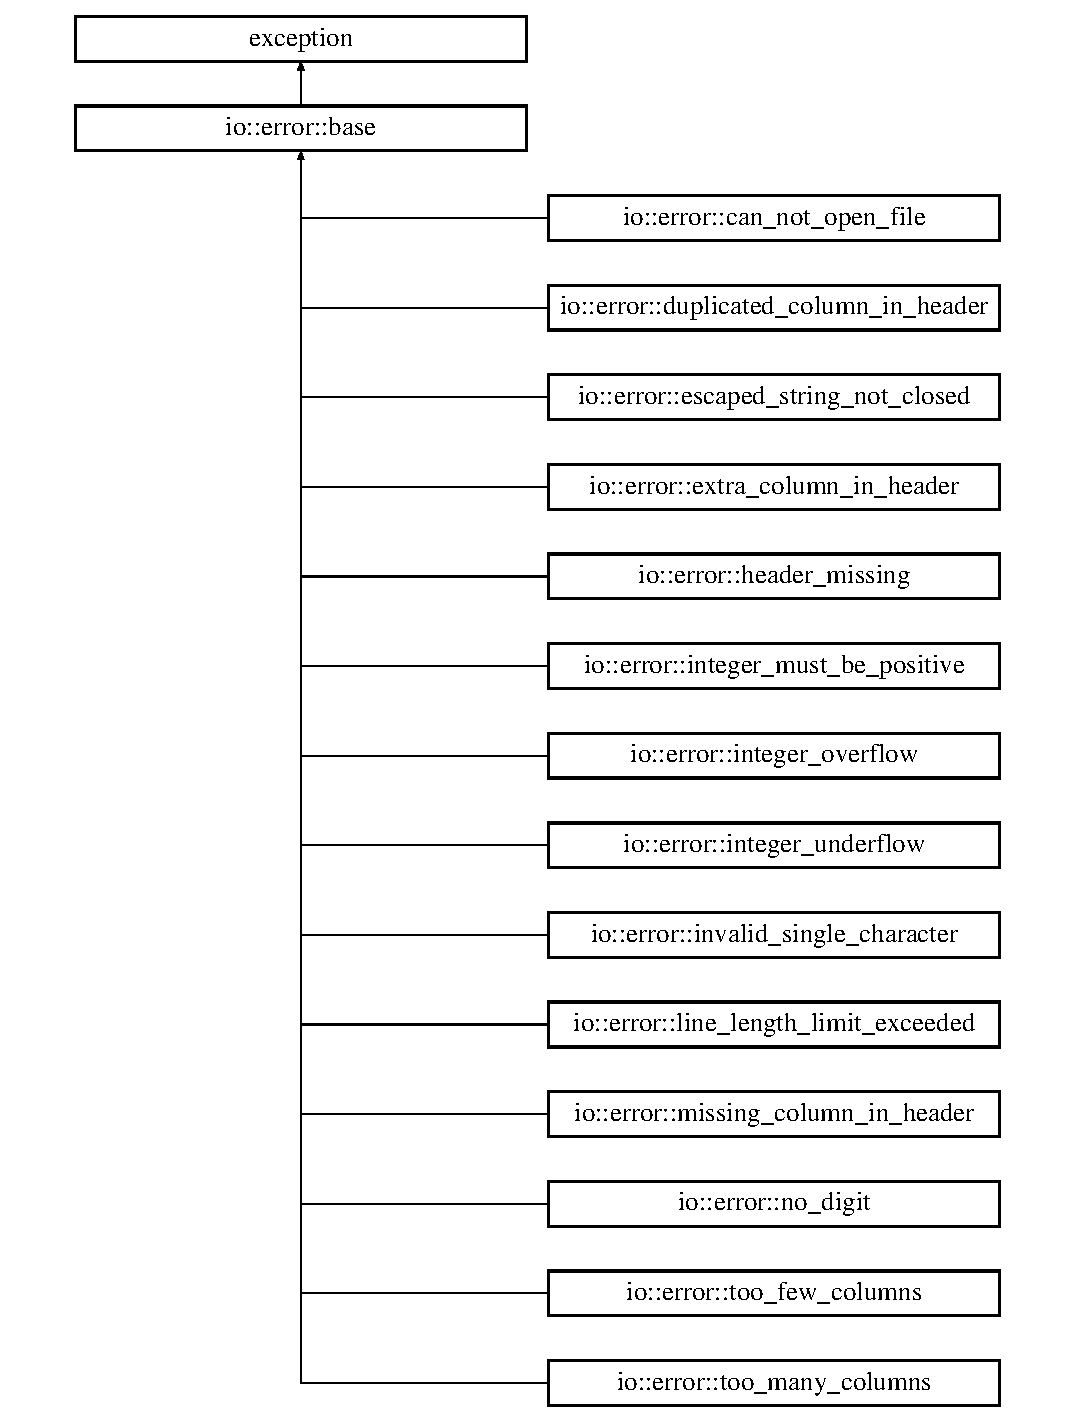
\includegraphics[height=12.000000cm]{structio_1_1error_1_1base}
\end{center}
\end{figure}
\subsection*{Public Member Functions}
\begin{DoxyCompactItemize}
\item 
\mbox{\Hypertarget{structio_1_1error_1_1base_a7d9ff6a31b716a24f056cf8a3e15191d}\label{structio_1_1error_1_1base_a7d9ff6a31b716a24f056cf8a3e15191d}} 
virtual void {\bfseries format\+\_\+error\+\_\+message} () const =0
\item 
\mbox{\Hypertarget{structio_1_1error_1_1base_a35483dfbe91cea45cfa7c5613e83e5ef}\label{structio_1_1error_1_1base_a35483dfbe91cea45cfa7c5613e83e5ef}} 
const char $\ast$ {\bfseries what} () const  throw ()
\end{DoxyCompactItemize}
\subsection*{Public Attributes}
\begin{DoxyCompactItemize}
\item 
\mbox{\Hypertarget{structio_1_1error_1_1base_a3be516c4636b7b61133968cb8081c885}\label{structio_1_1error_1_1base_a3be516c4636b7b61133968cb8081c885}} 
char {\bfseries error\+\_\+message\+\_\+buffer} \mbox{[}512\mbox{]}
\end{DoxyCompactItemize}


The documentation for this struct was generated from the following file\+:\begin{DoxyCompactItemize}
\item 
library/csv.\+h\end{DoxyCompactItemize}

\hypertarget{classio_1_1ByteSourceBase}{}\section{io\+:\+:Byte\+Source\+Base Class Reference}
\label{classio_1_1ByteSourceBase}\index{io\+::\+Byte\+Source\+Base@{io\+::\+Byte\+Source\+Base}}
Inheritance diagram for io\+:\+:Byte\+Source\+Base\+:\begin{figure}[H]
\begin{center}
\leavevmode
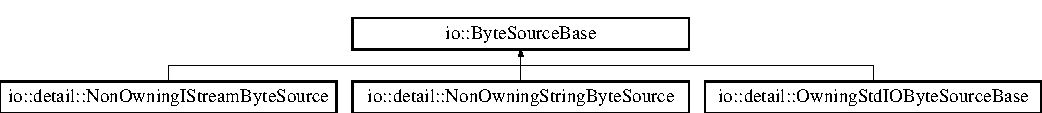
\includegraphics[height=1.517615cm]{classio_1_1ByteSourceBase}
\end{center}
\end{figure}
\subsection*{Public Member Functions}
\begin{DoxyCompactItemize}
\item 
\mbox{\Hypertarget{classio_1_1ByteSourceBase_a9598bcc869b79e44da07f0e6fa478615}\label{classio_1_1ByteSourceBase_a9598bcc869b79e44da07f0e6fa478615}} 
virtual int {\bfseries read} (char $\ast$buffer, int size)=0
\end{DoxyCompactItemize}


The documentation for this class was generated from the following file\+:\begin{DoxyCompactItemize}
\item 
library/csv.\+h\end{DoxyCompactItemize}

\hypertarget{structio_1_1error_1_1can__not__open__file}{}\section{io\+:\+:error\+:\+:can\+\_\+not\+\_\+open\+\_\+file Struct Reference}
\label{structio_1_1error_1_1can__not__open__file}\index{io\+::error\+::can\+\_\+not\+\_\+open\+\_\+file@{io\+::error\+::can\+\_\+not\+\_\+open\+\_\+file}}
Inheritance diagram for io\+:\+:error\+:\+:can\+\_\+not\+\_\+open\+\_\+file\+:\begin{figure}[H]
\begin{center}
\leavevmode
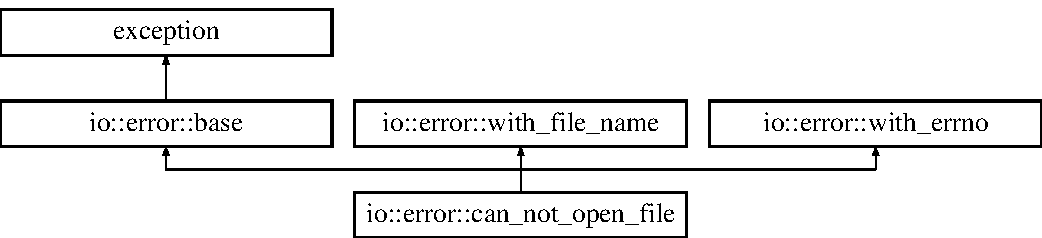
\includegraphics[height=3.000000cm]{structio_1_1error_1_1can__not__open__file}
\end{center}
\end{figure}
\subsection*{Public Member Functions}
\begin{DoxyCompactItemize}
\item 
\mbox{\Hypertarget{structio_1_1error_1_1can__not__open__file_a0249122edaf123e9fa4baabe8128806c}\label{structio_1_1error_1_1can__not__open__file_a0249122edaf123e9fa4baabe8128806c}} 
void {\bfseries format\+\_\+error\+\_\+message} () const
\end{DoxyCompactItemize}
\subsection*{Additional Inherited Members}


The documentation for this struct was generated from the following file\+:\begin{DoxyCompactItemize}
\item 
library/csv.\+h\end{DoxyCompactItemize}

\hypertarget{classclara_1_1clara}{}\section{clara\+:\+:clara Class Reference}
\label{classclara_1_1clara}\index{clara\+::clara@{clara\+::clara}}


The documentation for this class was generated from the following file\+:\begin{DoxyCompactItemize}
\item 
library/clara.\+h\end{DoxyCompactItemize}

\hypertarget{classclara_1_1cone__state}{}\section{clara\+:\+:cone\+\_\+state$<$ T $>$ Class Template Reference}
\label{classclara_1_1cone__state}\index{clara\+::cone\+\_\+state$<$ T $>$@{clara\+::cone\+\_\+state$<$ T $>$}}


A wrapper for the cone state.  




{\ttfamily \#include $<$cone\+\_\+state.\+h$>$}

\subsection*{Public Types}
\begin{DoxyCompactItemize}
\item 
\mbox{\Hypertarget{classclara_1_1cone__state_a74ce83ddac5e4056fd4bb1e7d217f9f8}\label{classclara_1_1cone__state_a74ce83ddac5e4056fd4bb1e7d217f9f8}} 
using \hyperlink{classclara_1_1cone__state_a74ce83ddac5e4056fd4bb1e7d217f9f8}{self\+\_\+t} = \hyperlink{classclara_1_1cone__state}{cone\+\_\+state}$<$ T $>$
\begin{DoxyCompactList}\small\item\em for convenience purposes \end{DoxyCompactList}\item 
\mbox{\Hypertarget{classclara_1_1cone__state_af16fa702d40bf1aa21315c5df376c797}\label{classclara_1_1cone__state_af16fa702d40bf1aa21315c5df376c797}} 
using {\bfseries coords\+\_\+t} = std\+::array$<$ T, 2 $>$
\end{DoxyCompactItemize}
\subsection*{Public Member Functions}
\begin{DoxyCompactItemize}
\item 
\mbox{\Hypertarget{classclara_1_1cone__state_ae8c7feebfc46bd183d93db3245c43a3d}\label{classclara_1_1cone__state_ae8c7feebfc46bd183d93db3245c43a3d}} 
\hyperlink{classclara_1_1cone__state_ae8c7feebfc46bd183d93db3245c43a3d}{cone\+\_\+state} (const \hyperlink{classclara_1_1cone__state_a74ce83ddac5e4056fd4bb1e7d217f9f8}{self\+\_\+t} \&other)=delete
\begin{DoxyCompactList}\small\item\em deleted copy constructor, we don\textquotesingle{}t want anybody to move or copy this object \end{DoxyCompactList}\item 
\mbox{\Hypertarget{classclara_1_1cone__state_ad70f9d4e537af05a549853f276813ce6}\label{classclara_1_1cone__state_ad70f9d4e537af05a549853f276813ce6}} 
\hyperlink{classclara_1_1cone__state_ad70f9d4e537af05a549853f276813ce6}{cone\+\_\+state} (const \hyperlink{classclara_1_1cone__state_a74ce83ddac5e4056fd4bb1e7d217f9f8}{self\+\_\+t} \&\&other)=delete
\begin{DoxyCompactList}\small\item\em deleted move constructor, we don\textquotesingle{}t want anybody to move or copy this object \end{DoxyCompactList}\item 
void \hyperlink{classclara_1_1cone__state_a7cd7364ca787c25b0ca333d0cb1c3081}{add\+\_\+observation} (T x, T y)
\begin{DoxyCompactList}\small\item\em Adds an observation of coordiantes to the cone state. \end{DoxyCompactList}\item 
\mbox{\Hypertarget{classclara_1_1cone__state_ae8642cde249796203a906df935e35f39}\label{classclara_1_1cone__state_ae8642cde249796203a906df935e35f39}} 
bool \hyperlink{classclara_1_1cone__state_ae8642cde249796203a906df935e35f39}{is\+\_\+modified} ()
\begin{DoxyCompactList}\small\item\em just for a naming convenience \end{DoxyCompactList}\item 
\mbox{\Hypertarget{classclara_1_1cone__state_a8cb6454f6a731f69d3e85382b0ae40b4}\label{classclara_1_1cone__state_a8cb6454f6a731f69d3e85382b0ae40b4}} 
void \hyperlink{classclara_1_1cone__state_a8cb6454f6a731f69d3e85382b0ae40b4}{update\+\_\+state} ()
\begin{DoxyCompactList}\small\item\em Updates the {\ttfamily \+\_\+mean\+\_\+vec}, {\ttfamily \+\_\+cov\+\_\+mat}, {\ttfamily \+\_\+det\+\_\+cov\+\_\+mat} and {\ttfamily \+\_\+inv\+\_\+cov\+\_\+mat} if {\ttfamily is\+\_\+modified} returns true These calculations have to be done in {\bfseries this exact order}, because they are all dependent on each other Results in a cached access to every member after recalculation for the current {\ttfamily \+\_\+observations} \end{DoxyCompactList}\item 
double \hyperlink{classclara_1_1cone__state_a331360538f2fc8ccaaa37db2a71cc1a8}{maximum\+\_\+likelihood\+\_\+estimate} (T x, T y)
\begin{DoxyCompactList}\small\item\em Maximum likelihood estimate for this parametrization Linearized gaussian multiplication for 2x2 matrizes of the mahalanobis distance in the exponent of {\ttfamily e} \end{DoxyCompactList}\end{DoxyCompactItemize}
\subsection*{Private Member Functions}
\begin{DoxyCompactItemize}
\item 
\mbox{\Hypertarget{classclara_1_1cone__state_ac9712fb4aee53df62da1cd320a45f813}\label{classclara_1_1cone__state_ac9712fb4aee53df62da1cd320a45f813}} 
void \hyperlink{classclara_1_1cone__state_ac9712fb4aee53df62da1cd320a45f813}{set\+\_\+modified} (bool b)
\begin{DoxyCompactList}\small\item\em setter for our modification flag, this is used to show if we got new information about our position Any access to {\ttfamily \+\_\+mean\+\_\+vec}, {\ttfamily \+\_\+cov\+\_\+mat}, {\ttfamily \+\_\+det\+\_\+cov\+\_\+mat} and {\ttfamily \+\_\+inv\+\_\+cov\+\_\+mat} triggers their recomputation via {\ttfamily \hyperlink{classclara_1_1cone__state_a8cb6454f6a731f69d3e85382b0ae40b4}{update\+\_\+state()}} \end{DoxyCompactList}\item 
const std\+::array$<$ T, 4 $>$ \& \hyperlink{classclara_1_1cone__state_a7a0584b86ba125a2c232f26d4d1e4a38}{get\+\_\+inv\+\_\+cov\+\_\+mat} ()
\begin{DoxyCompactList}\small\item\em This acces to {\ttfamily \+\_\+inv\+\_\+cov\+\_\+mat} can trigger a recalculation of the cone state. {\itshape Cached} \end{DoxyCompactList}\item 
\mbox{\Hypertarget{classclara_1_1cone__state_a5775993f75df93a3121c1fb53ef48777}\label{classclara_1_1cone__state_a5775993f75df93a3121c1fb53ef48777}} 
const T \& \hyperlink{classclara_1_1cone__state_a5775993f75df93a3121c1fb53ef48777}{get\+\_\+det\+\_\+cov\+\_\+mat} ()
\begin{DoxyCompactList}\small\item\em This access to {\ttfamily \+\_\+det\+\_\+cov\+\_\+mat} can trigger a recalulation of the cone state. {\itshape Cached} \end{DoxyCompactList}\item 
void \hyperlink{classclara_1_1cone__state_a7b0d6ab972d3d003eaad439c630c1c73}{update\+\_\+inv\+\_\+cov\+\_\+mat} ()
\begin{DoxyCompactList}\small\item\em Inverse matrix calculation of the 2x2 {\ttfamily \+\_\+cov\+\_\+mat}, saved in {\ttfamily \+\_\+inv\+\_\+cov\+\_\+mat} {\bfseries Invariant\+:} \end{DoxyCompactList}\item 
\mbox{\Hypertarget{classclara_1_1cone__state_ac04710abc3eba0e3688c70eaeab3f2ce}\label{classclara_1_1cone__state_ac04710abc3eba0e3688c70eaeab3f2ce}} 
void \hyperlink{classclara_1_1cone__state_ac04710abc3eba0e3688c70eaeab3f2ce}{update\+\_\+det\+\_\+cov\+\_\+mat} ()
\begin{DoxyCompactList}\small\item\em Cached determinant calculation of a 2x2 matrix {\ttfamily \+\_\+cov\+\_\+mat}, saved in {\ttfamily \+\_\+det\+\_\+cov\+\_\+mat} Property\+: {\ttfamily \+\_\+det\+\_\+cov\+\_\+mat} will never be 0, because the gaussian sampling in the EM algorithm is not defined for a zero covariance in all dimensions. We then set it to {\ttfamily 1} {\bfseries Invariant\+:} {\ttfamily \+\_\+cov\+\_\+mat} is up to date. \end{DoxyCompactList}\item 
void \hyperlink{classclara_1_1cone__state_ada683dbedcee79d84db8255ee5e71e6e}{update\+\_\+mean\+\_\+vec} ()
\begin{DoxyCompactList}\small\item\em Updates the {\ttfamily \+\_\+mean\+\_\+vec} with the current {\ttfamily \+\_\+observations} {\bfseries Invariant\+:} {\ttfamily \+\_\+observations} is up to date. \end{DoxyCompactList}\item 
void \hyperlink{classclara_1_1cone__state_a946bca664d068d7a82e3740eb736e948}{update\+\_\+cov\+\_\+mat} ()
\begin{DoxyCompactList}\small\item\em Updates the {\ttfamily \+\_\+cov\+\_\+mat} with the current {\ttfamily \+\_\+observations} and {\ttfamily \+\_\+mean\+\_\+vec} {\bfseries Invariant\+:} {\ttfamily \+\_\+mean\+\_\+vec}, {\ttfamily \+\_\+observations} is up to date. \end{DoxyCompactList}\end{DoxyCompactItemize}
\subsection*{Private Attributes}
\begin{DoxyCompactItemize}
\item 
\mbox{\Hypertarget{classclara_1_1cone__state_a0e08ed1150f22d7edffbcb2152cf4d29}\label{classclara_1_1cone__state_a0e08ed1150f22d7edffbcb2152cf4d29}} 
bool \hyperlink{classclara_1_1cone__state_a0e08ed1150f22d7edffbcb2152cf4d29}{\+\_\+modified}
\begin{DoxyCompactList}\small\item\em modification flag, if this is true, we need to recompute {\ttfamily \+\_\+cov\+\_\+mat}, {\ttfamily \+\_\+inv\+\_\+cov\+\_\+mat} and {\ttfamily \+\_\+mean\+\_\+vec}. {\ttfamily \hyperlink{classclara_1_1cone__state_a7cd7364ca787c25b0ca333d0cb1c3081}{add\+\_\+observation()}} triggers this \end{DoxyCompactList}\item 
std\+::vector$<$ coords\+\_\+t $>$ \hyperlink{classclara_1_1cone__state_ae5c8c1ba05533a80ab1874fb878888b9}{\+\_\+observations}
\begin{DoxyCompactList}\small\item\em List of the observations of this particular cone, {\ttfamily \hyperlink{classclara_1_1cone__state_a7cd7364ca787c25b0ca333d0cb1c3081}{add\+\_\+observation()}} can add elements to this list {\ttfamily \+\_\+observations} is preallocated in the constructor to a certain size. \end{DoxyCompactList}\item 
std\+::array$<$ T, 4 $>$ \hyperlink{classclara_1_1cone__state_a2a5e7dc2078a6d5ef80b1bac25354e2f}{\+\_\+cov\+\_\+mat}
\begin{DoxyCompactList}\small\item\em Linearized representation of a 2x2 matrix. \end{DoxyCompactList}\item 
std\+::array$<$ T, 4 $>$ \hyperlink{classclara_1_1cone__state_af36bb866c831dfc5b7b199d6434511f4}{\+\_\+inv\+\_\+cov\+\_\+mat}
\begin{DoxyCompactList}\small\item\em Linearized representation of a 2x2 matrix. \end{DoxyCompactList}\item 
\mbox{\Hypertarget{classclara_1_1cone__state_aa42f4654a82f825dc3b89d4ec0b03deb}\label{classclara_1_1cone__state_aa42f4654a82f825dc3b89d4ec0b03deb}} 
T \hyperlink{classclara_1_1cone__state_aa42f4654a82f825dc3b89d4ec0b03deb}{\+\_\+det\+\_\+cov\+\_\+mat}
\begin{DoxyCompactList}\small\item\em Determinand of \+\_\+cov\+\_\+mat. \end{DoxyCompactList}\item 
std\+::array$<$ T, 2 $>$ \hyperlink{classclara_1_1cone__state_abf600e69be6a3791caefb93b214bb3b5}{\+\_\+mean\+\_\+vec}
\begin{DoxyCompactList}\small\item\em mean vector of x and y (0 and 1 index respectivly) \end{DoxyCompactList}\end{DoxyCompactItemize}


\subsection{Detailed Description}
\subsubsection*{template$<$typename T$>$\newline
class clara\+::cone\+\_\+state$<$ T $>$}

A wrapper for the cone state. 

This class servers as the full knowledge base of a cone from the start of the detection We use this for the \href{data_association.h}{\tt data\+\_\+association} task, which in turn uses the \mbox{[}Expectation Maximization algorithm\mbox{]})(\href{https://en.wikipedia.org/wiki/Expectation%E2%80%93maximization_algorithm}{\tt https\+://en.\+wikipedia.\+org/wiki/\+Expectation\%\+E2\%80\%93maximization\+\_\+algorithm}) to associate detected cones to the known cones.

To do EM, we need to calculate the mean und covariance matrix over {\ttfamily x, y}. Because we know we only have a 2-\/dimensional state, we provide the needed functionality to do a gauss-\/sampling. See {\ttfamily \hyperlink{classclara_1_1cone__state_a7a0584b86ba125a2c232f26d4d1e4a38}{get\+\_\+inv\+\_\+cov\+\_\+mat()}} and {\ttfamily \hyperlink{classclara_1_1cone__state_a5775993f75df93a3121c1fb53ef48777}{get\+\_\+det\+\_\+cov\+\_\+mat()}}

Because of the assumption that new cones

Template arguments\+:
\begin{DoxyItemize}
\item {\ttfamily T} is the type of the interal coordinates
\end{DoxyItemize}

Restrictions\+:
\begin{DoxyItemize}
\item {\ttfamily T} has to be moveable
\end{DoxyItemize}

\begin{DoxyRefDesc}{Todo}
\item[\hyperlink{todo__todo000001}{Todo}]add {\ttfamily is\+\_\+integral} test for template {\ttfamily T} \end{DoxyRefDesc}


\subsection{Member Function Documentation}
\mbox{\Hypertarget{classclara_1_1cone__state_a7cd7364ca787c25b0ca333d0cb1c3081}\label{classclara_1_1cone__state_a7cd7364ca787c25b0ca333d0cb1c3081}} 
\index{clara\+::cone\+\_\+state@{clara\+::cone\+\_\+state}!add\+\_\+observation@{add\+\_\+observation}}
\index{add\+\_\+observation@{add\+\_\+observation}!clara\+::cone\+\_\+state@{clara\+::cone\+\_\+state}}
\subsubsection{\texorpdfstring{add\+\_\+observation()}{add\_observation()}}
{\footnotesize\ttfamily template$<$typename T $>$ \\
void \hyperlink{classclara_1_1cone__state}{clara\+::cone\+\_\+state}$<$ T $>$\+::add\+\_\+observation (\begin{DoxyParamCaption}\item[{T}]{x,  }\item[{T}]{y }\end{DoxyParamCaption})\hspace{0.3cm}{\ttfamily [inline]}}



Adds an observation of coordiantes to the cone state. 

This should be called if the EM algorithm determined with a sufficient probability that those coordiantes are in fact associated with this cone For the thoughful people, we use {\ttfamily \hyperlink{classclara_1_1cone__state_ac9712fb4aee53df62da1cd320a45f813}{set\+\_\+modified()}} and don\textquotesingle{}t recalculate the {\ttfamily \+\_\+cov\+\_\+mat} and {\ttfamily \+\_\+mean\+\_\+vec} because we can have multiple observations of the same cone at the same time This highly depends on the detection algorithm

\begin{DoxyRefDesc}{Todo}
\item[\hyperlink{todo__todo000002}{Todo}]test emplace\+\_\+back instead of push\+\_\+back 

test streaming mean / covariance functions so we don\textquotesingle{}t need to accumulate all observations \end{DoxyRefDesc}
\mbox{\Hypertarget{classclara_1_1cone__state_a7a0584b86ba125a2c232f26d4d1e4a38}\label{classclara_1_1cone__state_a7a0584b86ba125a2c232f26d4d1e4a38}} 
\index{clara\+::cone\+\_\+state@{clara\+::cone\+\_\+state}!get\+\_\+inv\+\_\+cov\+\_\+mat@{get\+\_\+inv\+\_\+cov\+\_\+mat}}
\index{get\+\_\+inv\+\_\+cov\+\_\+mat@{get\+\_\+inv\+\_\+cov\+\_\+mat}!clara\+::cone\+\_\+state@{clara\+::cone\+\_\+state}}
\subsubsection{\texorpdfstring{get\+\_\+inv\+\_\+cov\+\_\+mat()}{get\_inv\_cov\_mat()}}
{\footnotesize\ttfamily template$<$typename T $>$ \\
const std\+::array$<$T, 4$>$\& \hyperlink{classclara_1_1cone__state}{clara\+::cone\+\_\+state}$<$ T $>$\+::get\+\_\+inv\+\_\+cov\+\_\+mat (\begin{DoxyParamCaption}{ }\end{DoxyParamCaption})\hspace{0.3cm}{\ttfamily [inline]}, {\ttfamily [private]}}



This acces to {\ttfamily \+\_\+inv\+\_\+cov\+\_\+mat} can trigger a recalculation of the cone state. {\itshape Cached} 

\mbox{\Hypertarget{classclara_1_1cone__state_a331360538f2fc8ccaaa37db2a71cc1a8}\label{classclara_1_1cone__state_a331360538f2fc8ccaaa37db2a71cc1a8}} 
\index{clara\+::cone\+\_\+state@{clara\+::cone\+\_\+state}!maximum\+\_\+likelihood\+\_\+estimate@{maximum\+\_\+likelihood\+\_\+estimate}}
\index{maximum\+\_\+likelihood\+\_\+estimate@{maximum\+\_\+likelihood\+\_\+estimate}!clara\+::cone\+\_\+state@{clara\+::cone\+\_\+state}}
\subsubsection{\texorpdfstring{maximum\+\_\+likelihood\+\_\+estimate()}{maximum\_likelihood\_estimate()}}
{\footnotesize\ttfamily template$<$typename T $>$ \\
double \hyperlink{classclara_1_1cone__state}{clara\+::cone\+\_\+state}$<$ T $>$\+::maximum\+\_\+likelihood\+\_\+estimate (\begin{DoxyParamCaption}\item[{T}]{x,  }\item[{T}]{y }\end{DoxyParamCaption})\hspace{0.3cm}{\ttfamily [inline]}}



Maximum likelihood estimate for this parametrization Linearized gaussian multiplication for 2x2 matrizes of the mahalanobis distance in the exponent of {\ttfamily e} 

\begin{DoxyRefDesc}{Todo}
\item[\hyperlink{todo__todo000003}{Todo}]make a nice image for the explanation {\bfseries Invariant\+:} All the members are updated \end{DoxyRefDesc}
\mbox{\Hypertarget{classclara_1_1cone__state_a946bca664d068d7a82e3740eb736e948}\label{classclara_1_1cone__state_a946bca664d068d7a82e3740eb736e948}} 
\index{clara\+::cone\+\_\+state@{clara\+::cone\+\_\+state}!update\+\_\+cov\+\_\+mat@{update\+\_\+cov\+\_\+mat}}
\index{update\+\_\+cov\+\_\+mat@{update\+\_\+cov\+\_\+mat}!clara\+::cone\+\_\+state@{clara\+::cone\+\_\+state}}
\subsubsection{\texorpdfstring{update\+\_\+cov\+\_\+mat()}{update\_cov\_mat()}}
{\footnotesize\ttfamily template$<$typename T $>$ \\
void \hyperlink{classclara_1_1cone__state}{clara\+::cone\+\_\+state}$<$ T $>$\+::update\+\_\+cov\+\_\+mat (\begin{DoxyParamCaption}{ }\end{DoxyParamCaption})\hspace{0.3cm}{\ttfamily [inline]}, {\ttfamily [private]}}



Updates the {\ttfamily \+\_\+cov\+\_\+mat} with the current {\ttfamily \+\_\+observations} and {\ttfamily \+\_\+mean\+\_\+vec} {\bfseries Invariant\+:} {\ttfamily \+\_\+mean\+\_\+vec}, {\ttfamily \+\_\+observations} is up to date. 

\begin{DoxyRefDesc}{Todo}
\item[\hyperlink{todo__todo000005}{Todo}]parallelize this loop and test the performance time \end{DoxyRefDesc}
\mbox{\Hypertarget{classclara_1_1cone__state_a7b0d6ab972d3d003eaad439c630c1c73}\label{classclara_1_1cone__state_a7b0d6ab972d3d003eaad439c630c1c73}} 
\index{clara\+::cone\+\_\+state@{clara\+::cone\+\_\+state}!update\+\_\+inv\+\_\+cov\+\_\+mat@{update\+\_\+inv\+\_\+cov\+\_\+mat}}
\index{update\+\_\+inv\+\_\+cov\+\_\+mat@{update\+\_\+inv\+\_\+cov\+\_\+mat}!clara\+::cone\+\_\+state@{clara\+::cone\+\_\+state}}
\subsubsection{\texorpdfstring{update\+\_\+inv\+\_\+cov\+\_\+mat()}{update\_inv\_cov\_mat()}}
{\footnotesize\ttfamily template$<$typename T $>$ \\
void \hyperlink{classclara_1_1cone__state}{clara\+::cone\+\_\+state}$<$ T $>$\+::update\+\_\+inv\+\_\+cov\+\_\+mat (\begin{DoxyParamCaption}{ }\end{DoxyParamCaption})\hspace{0.3cm}{\ttfamily [inline]}, {\ttfamily [private]}}



Inverse matrix calculation of the 2x2 {\ttfamily \+\_\+cov\+\_\+mat}, saved in {\ttfamily \+\_\+inv\+\_\+cov\+\_\+mat} {\bfseries Invariant\+:} 


\begin{DoxyItemize}
\item {\ttfamily \+\_\+det\+\_\+cov\+\_\+mat} and {\ttfamily \+\_\+cov\+\_\+mat} is up to date
\item {\ttfamily \+\_\+det\+\_\+cov\+\_\+mat} != 0, this is taken care of in {\ttfamily \hyperlink{classclara_1_1cone__state_ac04710abc3eba0e3688c70eaeab3f2ce}{update\+\_\+det\+\_\+cov\+\_\+mat()}} 
\end{DoxyItemize}\mbox{\Hypertarget{classclara_1_1cone__state_ada683dbedcee79d84db8255ee5e71e6e}\label{classclara_1_1cone__state_ada683dbedcee79d84db8255ee5e71e6e}} 
\index{clara\+::cone\+\_\+state@{clara\+::cone\+\_\+state}!update\+\_\+mean\+\_\+vec@{update\+\_\+mean\+\_\+vec}}
\index{update\+\_\+mean\+\_\+vec@{update\+\_\+mean\+\_\+vec}!clara\+::cone\+\_\+state@{clara\+::cone\+\_\+state}}
\subsubsection{\texorpdfstring{update\+\_\+mean\+\_\+vec()}{update\_mean\_vec()}}
{\footnotesize\ttfamily template$<$typename T $>$ \\
void \hyperlink{classclara_1_1cone__state}{clara\+::cone\+\_\+state}$<$ T $>$\+::update\+\_\+mean\+\_\+vec (\begin{DoxyParamCaption}{ }\end{DoxyParamCaption})\hspace{0.3cm}{\ttfamily [inline]}, {\ttfamily [private]}}



Updates the {\ttfamily \+\_\+mean\+\_\+vec} with the current {\ttfamily \+\_\+observations} {\bfseries Invariant\+:} {\ttfamily \+\_\+observations} is up to date. 

\begin{DoxyRefDesc}{Todo}
\item[\hyperlink{todo__todo000004}{Todo}]parallelize this loop and test the performance time \end{DoxyRefDesc}


\subsection{Member Data Documentation}
\mbox{\Hypertarget{classclara_1_1cone__state_a2a5e7dc2078a6d5ef80b1bac25354e2f}\label{classclara_1_1cone__state_a2a5e7dc2078a6d5ef80b1bac25354e2f}} 
\index{clara\+::cone\+\_\+state@{clara\+::cone\+\_\+state}!\+\_\+cov\+\_\+mat@{\+\_\+cov\+\_\+mat}}
\index{\+\_\+cov\+\_\+mat@{\+\_\+cov\+\_\+mat}!clara\+::cone\+\_\+state@{clara\+::cone\+\_\+state}}
\subsubsection{\texorpdfstring{\+\_\+cov\+\_\+mat}{\_cov\_mat}}
{\footnotesize\ttfamily template$<$typename T $>$ \\
std\+::array$<$T, 4$>$ \hyperlink{classclara_1_1cone__state}{clara\+::cone\+\_\+state}$<$ T $>$\+::\+\_\+cov\+\_\+mat\hspace{0.3cm}{\ttfamily [private]}}



Linearized representation of a 2x2 matrix. 


\begin{DoxyCode}
a = \hyperlink{classclara_1_1cone__state_a2a5e7dc2078a6d5ef80b1bac25354e2f}{\_cov\_mat}[0];
b = \hyperlink{classclara_1_1cone__state_a2a5e7dc2078a6d5ef80b1bac25354e2f}{\_cov\_mat}[1];
c = \hyperlink{classclara_1_1cone__state_a2a5e7dc2078a6d5ef80b1bac25354e2f}{\_cov\_mat}[2];
d = \hyperlink{classclara_1_1cone__state_a2a5e7dc2078a6d5ef80b1bac25354e2f}{\_cov\_mat}[3];
\end{DoxyCode}



\begin{DoxyCode}
[ [ a, b ]
 ,[ c, d ] ]
\end{DoxyCode}
 \mbox{\Hypertarget{classclara_1_1cone__state_af36bb866c831dfc5b7b199d6434511f4}\label{classclara_1_1cone__state_af36bb866c831dfc5b7b199d6434511f4}} 
\index{clara\+::cone\+\_\+state@{clara\+::cone\+\_\+state}!\+\_\+inv\+\_\+cov\+\_\+mat@{\+\_\+inv\+\_\+cov\+\_\+mat}}
\index{\+\_\+inv\+\_\+cov\+\_\+mat@{\+\_\+inv\+\_\+cov\+\_\+mat}!clara\+::cone\+\_\+state@{clara\+::cone\+\_\+state}}
\subsubsection{\texorpdfstring{\+\_\+inv\+\_\+cov\+\_\+mat}{\_inv\_cov\_mat}}
{\footnotesize\ttfamily template$<$typename T $>$ \\
std\+::array$<$T, 4$>$ \hyperlink{classclara_1_1cone__state}{clara\+::cone\+\_\+state}$<$ T $>$\+::\+\_\+inv\+\_\+cov\+\_\+mat\hspace{0.3cm}{\ttfamily [private]}}



Linearized representation of a 2x2 matrix. 


\begin{DoxyCode}
a = \hyperlink{classclara_1_1cone__state_af36bb866c831dfc5b7b199d6434511f4}{\_inv\_cov\_mat}[0];
b = \hyperlink{classclara_1_1cone__state_af36bb866c831dfc5b7b199d6434511f4}{\_inv\_cov\_mat}[1];
c = \hyperlink{classclara_1_1cone__state_af36bb866c831dfc5b7b199d6434511f4}{\_inv\_cov\_mat}[2];
d = \hyperlink{classclara_1_1cone__state_af36bb866c831dfc5b7b199d6434511f4}{\_inv\_cov\_mat}[3];
\end{DoxyCode}



\begin{DoxyCode}
[ [ a, b ]
 ,[ c, d ] ]
\end{DoxyCode}
 \mbox{\Hypertarget{classclara_1_1cone__state_abf600e69be6a3791caefb93b214bb3b5}\label{classclara_1_1cone__state_abf600e69be6a3791caefb93b214bb3b5}} 
\index{clara\+::cone\+\_\+state@{clara\+::cone\+\_\+state}!\+\_\+mean\+\_\+vec@{\+\_\+mean\+\_\+vec}}
\index{\+\_\+mean\+\_\+vec@{\+\_\+mean\+\_\+vec}!clara\+::cone\+\_\+state@{clara\+::cone\+\_\+state}}
\subsubsection{\texorpdfstring{\+\_\+mean\+\_\+vec}{\_mean\_vec}}
{\footnotesize\ttfamily template$<$typename T $>$ \\
std\+::array$<$T, 2$>$ \hyperlink{classclara_1_1cone__state}{clara\+::cone\+\_\+state}$<$ T $>$\+::\+\_\+mean\+\_\+vec\hspace{0.3cm}{\ttfamily [private]}}



mean vector of x and y (0 and 1 index respectivly) 


\begin{DoxyCode}
x = \hyperlink{classclara_1_1cone__state_abf600e69be6a3791caefb93b214bb3b5}{\_mean\_vec}[0];
y = \hyperlink{classclara_1_1cone__state_abf600e69be6a3791caefb93b214bb3b5}{\_mean\_vec}[1];
\end{DoxyCode}
 \mbox{\Hypertarget{classclara_1_1cone__state_ae5c8c1ba05533a80ab1874fb878888b9}\label{classclara_1_1cone__state_ae5c8c1ba05533a80ab1874fb878888b9}} 
\index{clara\+::cone\+\_\+state@{clara\+::cone\+\_\+state}!\+\_\+observations@{\+\_\+observations}}
\index{\+\_\+observations@{\+\_\+observations}!clara\+::cone\+\_\+state@{clara\+::cone\+\_\+state}}
\subsubsection{\texorpdfstring{\+\_\+observations}{\_observations}}
{\footnotesize\ttfamily template$<$typename T $>$ \\
std\+::vector$<$coords\+\_\+t$>$ \hyperlink{classclara_1_1cone__state}{clara\+::cone\+\_\+state}$<$ T $>$\+::\+\_\+observations\hspace{0.3cm}{\ttfamily [private]}}



List of the observations of this particular cone, {\ttfamily \hyperlink{classclara_1_1cone__state_a7cd7364ca787c25b0ca333d0cb1c3081}{add\+\_\+observation()}} can add elements to this list {\ttfamily \+\_\+observations} is preallocated in the constructor to a certain size. 

\begin{DoxyRefDesc}{Todo}
\item[\hyperlink{todo__todo000006}{Todo}]make the preallocation configurable \end{DoxyRefDesc}


The documentation for this class was generated from the following file\+:\begin{DoxyCompactItemize}
\item 
library/cone\+\_\+state.\+h\end{DoxyCompactItemize}

\hypertarget{classio_1_1CSVReader}{}\section{io\+:\+:C\+S\+V\+Reader$<$ column\+\_\+count, trim\+\_\+policy, quote\+\_\+policy, overflow\+\_\+policy, comment\+\_\+policy $>$ Class Template Reference}
\label{classio_1_1CSVReader}\index{io\+::\+C\+S\+V\+Reader$<$ column\+\_\+count, trim\+\_\+policy, quote\+\_\+policy, overflow\+\_\+policy, comment\+\_\+policy $>$@{io\+::\+C\+S\+V\+Reader$<$ column\+\_\+count, trim\+\_\+policy, quote\+\_\+policy, overflow\+\_\+policy, comment\+\_\+policy $>$}}
\subsection*{Public Member Functions}
\begin{DoxyCompactItemize}
\item 
\mbox{\Hypertarget{classio_1_1CSVReader_a0507ac5abe201969a15df76795e13c28}\label{classio_1_1CSVReader_a0507ac5abe201969a15df76795e13c28}} 
{\bfseries C\+S\+V\+Reader} (const \hyperlink{classio_1_1CSVReader}{C\+S\+V\+Reader} \&)=delete
\item 
\mbox{\Hypertarget{classio_1_1CSVReader_a37046e6629cf4254037c14440f14141d}\label{classio_1_1CSVReader_a37046e6629cf4254037c14440f14141d}} 
\hyperlink{classio_1_1CSVReader}{C\+S\+V\+Reader} \& {\bfseries operator=} (const \hyperlink{classio_1_1CSVReader}{C\+S\+V\+Reader} \&)
\item 
\mbox{\Hypertarget{classio_1_1CSVReader_a189debf95672e7cd7582e9f73d7203e5}\label{classio_1_1CSVReader_a189debf95672e7cd7582e9f73d7203e5}} 
{\footnotesize template$<$class ... Args$>$ }\\{\bfseries C\+S\+V\+Reader} (Args \&\&...args)
\item 
\mbox{\Hypertarget{classio_1_1CSVReader_a9fec7797cb27f64360cc48adc5f32c72}\label{classio_1_1CSVReader_a9fec7797cb27f64360cc48adc5f32c72}} 
char $\ast$ {\bfseries next\+\_\+line} ()
\item 
\mbox{\Hypertarget{classio_1_1CSVReader_a9fad9ae02aa243dba6bc78156c5ce7e5}\label{classio_1_1CSVReader_a9fad9ae02aa243dba6bc78156c5ce7e5}} 
{\footnotesize template$<$class ... Col\+Names$>$ }\\void {\bfseries read\+\_\+header} (ignore\+\_\+column ignore\+\_\+policy, Col\+Names...\+cols)
\item 
\mbox{\Hypertarget{classio_1_1CSVReader_ab68eedff1bd59a49fa4ddb160dff94e0}\label{classio_1_1CSVReader_ab68eedff1bd59a49fa4ddb160dff94e0}} 
{\footnotesize template$<$class ... Col\+Names$>$ }\\void {\bfseries set\+\_\+header} (Col\+Names...\+cols)
\item 
\mbox{\Hypertarget{classio_1_1CSVReader_aaba91fff6faea12e451943e8d32a5a17}\label{classio_1_1CSVReader_aaba91fff6faea12e451943e8d32a5a17}} 
bool {\bfseries has\+\_\+column} (const std\+::string \&name) const
\item 
\mbox{\Hypertarget{classio_1_1CSVReader_a4096c1e43a4fba2b4f5ae21d047b5fbc}\label{classio_1_1CSVReader_a4096c1e43a4fba2b4f5ae21d047b5fbc}} 
void {\bfseries set\+\_\+file\+\_\+name} (const std\+::string \&file\+\_\+name)
\item 
\mbox{\Hypertarget{classio_1_1CSVReader_a5f1dc083a8fa8661f5ecdcf6aebc7b24}\label{classio_1_1CSVReader_a5f1dc083a8fa8661f5ecdcf6aebc7b24}} 
void {\bfseries set\+\_\+file\+\_\+name} (const char $\ast$file\+\_\+name)
\item 
\mbox{\Hypertarget{classio_1_1CSVReader_abc6321895152f5a34959b499da6512ee}\label{classio_1_1CSVReader_abc6321895152f5a34959b499da6512ee}} 
const char $\ast$ {\bfseries get\+\_\+truncated\+\_\+file\+\_\+name} () const
\item 
\mbox{\Hypertarget{classio_1_1CSVReader_a1303bd6a2eb0d3d7c743212e52839ac4}\label{classio_1_1CSVReader_a1303bd6a2eb0d3d7c743212e52839ac4}} 
void {\bfseries set\+\_\+file\+\_\+line} (unsigned file\+\_\+line)
\item 
\mbox{\Hypertarget{classio_1_1CSVReader_a065f805596018d1568b81152e6a22e0c}\label{classio_1_1CSVReader_a065f805596018d1568b81152e6a22e0c}} 
unsigned {\bfseries get\+\_\+file\+\_\+line} () const
\item 
\mbox{\Hypertarget{classio_1_1CSVReader_a61ecdcaa62c024bf97c4e5d133478d7e}\label{classio_1_1CSVReader_a61ecdcaa62c024bf97c4e5d133478d7e}} 
{\footnotesize template$<$class ... Col\+Type$>$ }\\bool {\bfseries read\+\_\+row} (Col\+Type \&...cols)
\end{DoxyCompactItemize}
\subsection*{Private Member Functions}
\begin{DoxyCompactItemize}
\item 
\mbox{\Hypertarget{classio_1_1CSVReader_af0f3df423977925fd22acadbdbc4cdcd}\label{classio_1_1CSVReader_af0f3df423977925fd22acadbdbc4cdcd}} 
{\footnotesize template$<$class ... Col\+Names$>$ }\\void {\bfseries set\+\_\+column\+\_\+names} (std\+::string s, Col\+Names...\+cols)
\item 
\mbox{\Hypertarget{classio_1_1CSVReader_a48a56e02ae597ae3506e1b24dc0718ef}\label{classio_1_1CSVReader_a48a56e02ae597ae3506e1b24dc0718ef}} 
void {\bfseries set\+\_\+column\+\_\+names} ()
\item 
\mbox{\Hypertarget{classio_1_1CSVReader_ada16395fbaedad5fcda248b50cd12da0}\label{classio_1_1CSVReader_ada16395fbaedad5fcda248b50cd12da0}} 
void {\bfseries parse\+\_\+helper} (std\+::size\+\_\+t)
\item 
\mbox{\Hypertarget{classio_1_1CSVReader_a6e2cb67ff14a62cee48fb9042c1bfff9}\label{classio_1_1CSVReader_a6e2cb67ff14a62cee48fb9042c1bfff9}} 
{\footnotesize template$<$class T , class ... Col\+Type$>$ }\\void {\bfseries parse\+\_\+helper} (std\+::size\+\_\+t r, T \&t, Col\+Type \&...cols)
\end{DoxyCompactItemize}
\subsection*{Private Attributes}
\begin{DoxyCompactItemize}
\item 
\mbox{\Hypertarget{classio_1_1CSVReader_a26da3892b5c4606617d9daadc0886501}\label{classio_1_1CSVReader_a26da3892b5c4606617d9daadc0886501}} 
\hyperlink{classio_1_1LineReader}{Line\+Reader} {\bfseries in}
\item 
\mbox{\Hypertarget{classio_1_1CSVReader_a48ab5773a4295f7969453838b4115e42}\label{classio_1_1CSVReader_a48ab5773a4295f7969453838b4115e42}} 
char $\ast$ {\bfseries row} \mbox{[}column\+\_\+count\mbox{]}
\item 
\mbox{\Hypertarget{classio_1_1CSVReader_a7b97f929cea543f83e61173ea435fdde}\label{classio_1_1CSVReader_a7b97f929cea543f83e61173ea435fdde}} 
std\+::string {\bfseries column\+\_\+names} \mbox{[}column\+\_\+count\mbox{]}
\item 
\mbox{\Hypertarget{classio_1_1CSVReader_a1a59e51b74c2d6056821a5e499379884}\label{classio_1_1CSVReader_a1a59e51b74c2d6056821a5e499379884}} 
std\+::vector$<$ int $>$ {\bfseries col\+\_\+order}
\end{DoxyCompactItemize}


The documentation for this class was generated from the following file\+:\begin{DoxyCompactItemize}
\item 
library/csv.\+h\end{DoxyCompactItemize}

\hypertarget{classclara_1_1data__association}{}\section{clara\+:\+:data\+\_\+association$<$ N $>$ Class Template Reference}
\label{classclara_1_1data__association}\index{clara\+::data\+\_\+association$<$ N $>$@{clara\+::data\+\_\+association$<$ N $>$}}


A class which handles the data association task for C\+L\+A\+RA.  




{\ttfamily \#include $<$data\+\_\+association.\+h$>$}

\subsection*{Public Attributes}
\begin{DoxyCompactItemize}
\item 
\mbox{\Hypertarget{classclara_1_1data__association_a50e3471d0e0ae81acb13596e07c8b154}\label{classclara_1_1data__association_a50e3471d0e0ae81acb13596e07c8b154}} 
std\+::array$<$ \hyperlink{classclara_1_1data__association_a8bd65eee5fba8dcaa35d96b1c3c6daa2}{cone\+\_\+data}, N $>$ {\bfseries cone\+\_\+states}
\end{DoxyCompactItemize}
\subsection*{Private Types}
\begin{DoxyCompactItemize}
\item 
\mbox{\Hypertarget{classclara_1_1data__association_a8bd65eee5fba8dcaa35d96b1c3c6daa2}\label{classclara_1_1data__association_a8bd65eee5fba8dcaa35d96b1c3c6daa2}} 
using \hyperlink{classclara_1_1data__association_a8bd65eee5fba8dcaa35d96b1c3c6daa2}{cone\+\_\+data} = std\+::tuple$<$ double, double $>$
\begin{DoxyCompactList}\small\item\em {\ttfamily x} and {\ttfamily y} position \end{DoxyCompactList}\end{DoxyCompactItemize}


\subsection{Detailed Description}
\subsubsection*{template$<$size\+\_\+t N$>$\newline
class clara\+::data\+\_\+association$<$ N $>$}

A class which handles the data association task for C\+L\+A\+RA. 

The task of clara is to return the {\itshape best} estimate of the current world position

To do this, we detect cones based on some sensors which return\+:
\begin{DoxyItemize}
\item {\bfseries relative distance} to the current position
\item {\bfseries yaw angle} to the car direction. This is in the range of\begin{DoxyRefDesc}{Todo}
\item[\hyperlink{todo__todo000007}{Todo}]ask sheldon for yaw angle\end{DoxyRefDesc}

\end{DoxyItemize}

Cones are saved by their absolute position (x,y), based on the starting point of the car (usually {\ttfamily (0,0)})

Template arguments\+:
\begin{DoxyItemize}
\item {\ttfamily N} = maximum amount of cones which we\textquotesingle{}ll be able to identify 
\end{DoxyItemize}

The documentation for this class was generated from the following file\+:\begin{DoxyCompactItemize}
\item 
library/data\+\_\+association.\+h\end{DoxyCompactItemize}

\hypertarget{structio_1_1double__quote__escape}{}\section{io\+:\+:double\+\_\+quote\+\_\+escape$<$ sep, quote $>$ Struct Template Reference}
\label{structio_1_1double__quote__escape}\index{io\+::double\+\_\+quote\+\_\+escape$<$ sep, quote $>$@{io\+::double\+\_\+quote\+\_\+escape$<$ sep, quote $>$}}
\subsection*{Static Public Member Functions}
\begin{DoxyCompactItemize}
\item 
\mbox{\Hypertarget{structio_1_1double__quote__escape_a30070914039ca8a20f716fbf53d68c41}\label{structio_1_1double__quote__escape_a30070914039ca8a20f716fbf53d68c41}} 
static const char $\ast$ {\bfseries find\+\_\+next\+\_\+column\+\_\+end} (const char $\ast$col\+\_\+begin)
\item 
\mbox{\Hypertarget{structio_1_1double__quote__escape_a02e332751916fbdb7b35c238d690e580}\label{structio_1_1double__quote__escape_a02e332751916fbdb7b35c238d690e580}} 
static void {\bfseries unescape} (char $\ast$\&col\+\_\+begin, char $\ast$\&col\+\_\+end)
\end{DoxyCompactItemize}


The documentation for this struct was generated from the following file\+:\begin{DoxyCompactItemize}
\item 
library/csv.\+h\end{DoxyCompactItemize}

\hypertarget{structio_1_1error_1_1duplicated__column__in__header}{}\section{io\+:\+:error\+:\+:duplicated\+\_\+column\+\_\+in\+\_\+header Struct Reference}
\label{structio_1_1error_1_1duplicated__column__in__header}\index{io\+::error\+::duplicated\+\_\+column\+\_\+in\+\_\+header@{io\+::error\+::duplicated\+\_\+column\+\_\+in\+\_\+header}}
Inheritance diagram for io\+:\+:error\+:\+:duplicated\+\_\+column\+\_\+in\+\_\+header\+:\begin{figure}[H]
\begin{center}
\leavevmode
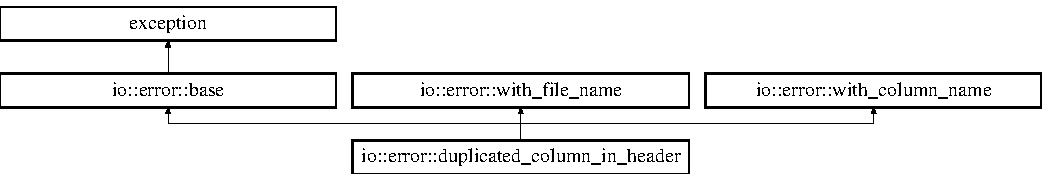
\includegraphics[height=2.333333cm]{structio_1_1error_1_1duplicated__column__in__header}
\end{center}
\end{figure}
\subsection*{Public Member Functions}
\begin{DoxyCompactItemize}
\item 
\mbox{\Hypertarget{structio_1_1error_1_1duplicated__column__in__header_a213825695d770d3ee2ee7bb9a2bfa818}\label{structio_1_1error_1_1duplicated__column__in__header_a213825695d770d3ee2ee7bb9a2bfa818}} 
void {\bfseries format\+\_\+error\+\_\+message} () const
\end{DoxyCompactItemize}
\subsection*{Additional Inherited Members}


The documentation for this struct was generated from the following file\+:\begin{DoxyCompactItemize}
\item 
library/csv.\+h\end{DoxyCompactItemize}

\hypertarget{structio_1_1empty__line__comment}{}\section{io\+:\+:empty\+\_\+line\+\_\+comment Struct Reference}
\label{structio_1_1empty__line__comment}\index{io\+::empty\+\_\+line\+\_\+comment@{io\+::empty\+\_\+line\+\_\+comment}}
\subsection*{Static Public Member Functions}
\begin{DoxyCompactItemize}
\item 
\mbox{\Hypertarget{structio_1_1empty__line__comment_a88e2cee044a9aafabf3e2a0e64fa5289}\label{structio_1_1empty__line__comment_a88e2cee044a9aafabf3e2a0e64fa5289}} 
static bool {\bfseries is\+\_\+comment} (const char $\ast$line)
\end{DoxyCompactItemize}


The documentation for this struct was generated from the following file\+:\begin{DoxyCompactItemize}
\item 
library/csv.\+h\end{DoxyCompactItemize}

\hypertarget{structio_1_1error_1_1escaped__string__not__closed}{}\section{io\+:\+:error\+:\+:escaped\+\_\+string\+\_\+not\+\_\+closed Struct Reference}
\label{structio_1_1error_1_1escaped__string__not__closed}\index{io\+::error\+::escaped\+\_\+string\+\_\+not\+\_\+closed@{io\+::error\+::escaped\+\_\+string\+\_\+not\+\_\+closed}}
Inheritance diagram for io\+:\+:error\+:\+:escaped\+\_\+string\+\_\+not\+\_\+closed\+:\begin{figure}[H]
\begin{center}
\leavevmode
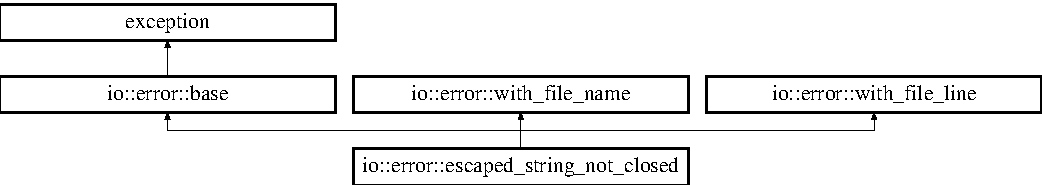
\includegraphics[height=2.488889cm]{structio_1_1error_1_1escaped__string__not__closed}
\end{center}
\end{figure}
\subsection*{Public Member Functions}
\begin{DoxyCompactItemize}
\item 
\mbox{\Hypertarget{structio_1_1error_1_1escaped__string__not__closed_a696911cd3cfaf8a30a728101b076028d}\label{structio_1_1error_1_1escaped__string__not__closed_a696911cd3cfaf8a30a728101b076028d}} 
void {\bfseries format\+\_\+error\+\_\+message} () const
\end{DoxyCompactItemize}
\subsection*{Additional Inherited Members}


The documentation for this struct was generated from the following file\+:\begin{DoxyCompactItemize}
\item 
library/csv.\+h\end{DoxyCompactItemize}

\hypertarget{structio_1_1error_1_1extra__column__in__header}{}\section{io\+:\+:error\+:\+:extra\+\_\+column\+\_\+in\+\_\+header Struct Reference}
\label{structio_1_1error_1_1extra__column__in__header}\index{io\+::error\+::extra\+\_\+column\+\_\+in\+\_\+header@{io\+::error\+::extra\+\_\+column\+\_\+in\+\_\+header}}
Inheritance diagram for io\+:\+:error\+:\+:extra\+\_\+column\+\_\+in\+\_\+header\+:\begin{figure}[H]
\begin{center}
\leavevmode
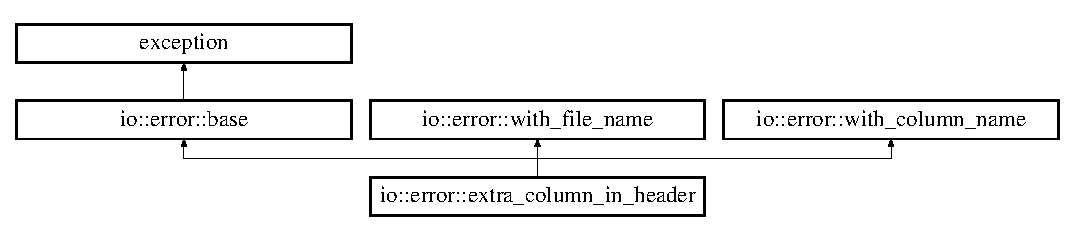
\includegraphics[height=2.666667cm]{structio_1_1error_1_1extra__column__in__header}
\end{center}
\end{figure}
\subsection*{Public Member Functions}
\begin{DoxyCompactItemize}
\item 
\mbox{\Hypertarget{structio_1_1error_1_1extra__column__in__header_ab7bb962a470c429206c51729fbf114dd}\label{structio_1_1error_1_1extra__column__in__header_ab7bb962a470c429206c51729fbf114dd}} 
void {\bfseries format\+\_\+error\+\_\+message} () const
\end{DoxyCompactItemize}
\subsection*{Additional Inherited Members}


The documentation for this struct was generated from the following file\+:\begin{DoxyCompactItemize}
\item 
library/csv.\+h\end{DoxyCompactItemize}

\hypertarget{structio_1_1error_1_1header__missing}{}\section{io\+:\+:error\+:\+:header\+\_\+missing Struct Reference}
\label{structio_1_1error_1_1header__missing}\index{io\+::error\+::header\+\_\+missing@{io\+::error\+::header\+\_\+missing}}
Inheritance diagram for io\+:\+:error\+:\+:header\+\_\+missing\+:\begin{figure}[H]
\begin{center}
\leavevmode
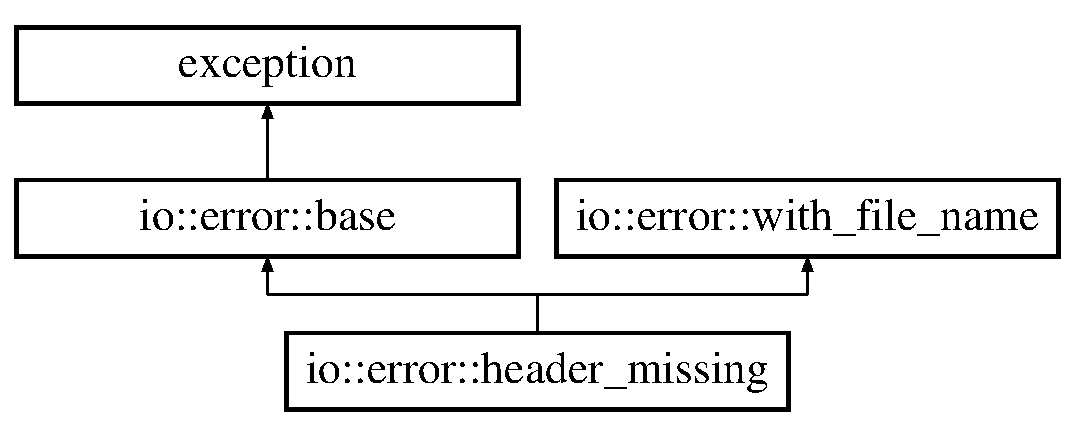
\includegraphics[height=3.000000cm]{structio_1_1error_1_1header__missing}
\end{center}
\end{figure}
\subsection*{Public Member Functions}
\begin{DoxyCompactItemize}
\item 
\mbox{\Hypertarget{structio_1_1error_1_1header__missing_ae130d632556617cf136cc4392b517b30}\label{structio_1_1error_1_1header__missing_ae130d632556617cf136cc4392b517b30}} 
void {\bfseries format\+\_\+error\+\_\+message} () const
\end{DoxyCompactItemize}
\subsection*{Additional Inherited Members}


The documentation for this struct was generated from the following file\+:\begin{DoxyCompactItemize}
\item 
library/csv.\+h\end{DoxyCompactItemize}

\hypertarget{structio_1_1ignore__overflow}{}\section{io\+:\+:ignore\+\_\+overflow Struct Reference}
\label{structio_1_1ignore__overflow}\index{io\+::ignore\+\_\+overflow@{io\+::ignore\+\_\+overflow}}
\subsection*{Static Public Member Functions}
\begin{DoxyCompactItemize}
\item 
\mbox{\Hypertarget{structio_1_1ignore__overflow_aed3e5026cfa7157ea9270ae377d1026b}\label{structio_1_1ignore__overflow_aed3e5026cfa7157ea9270ae377d1026b}} 
{\footnotesize template$<$class T $>$ }\\static void {\bfseries on\+\_\+overflow} (T \&)
\item 
\mbox{\Hypertarget{structio_1_1ignore__overflow_aece692f7a20933149ec99aa1f97458ad}\label{structio_1_1ignore__overflow_aece692f7a20933149ec99aa1f97458ad}} 
{\footnotesize template$<$class T $>$ }\\static void {\bfseries on\+\_\+underflow} (T \&)
\end{DoxyCompactItemize}


The documentation for this struct was generated from the following file\+:\begin{DoxyCompactItemize}
\item 
library/csv.\+h\end{DoxyCompactItemize}

\hypertarget{structio_1_1error_1_1integer__must__be__positive}{}\section{io\+:\+:error\+:\+:integer\+\_\+must\+\_\+be\+\_\+positive Struct Reference}
\label{structio_1_1error_1_1integer__must__be__positive}\index{io\+::error\+::integer\+\_\+must\+\_\+be\+\_\+positive@{io\+::error\+::integer\+\_\+must\+\_\+be\+\_\+positive}}
Inheritance diagram for io\+:\+:error\+:\+:integer\+\_\+must\+\_\+be\+\_\+positive\+:\begin{figure}[H]
\begin{center}
\leavevmode
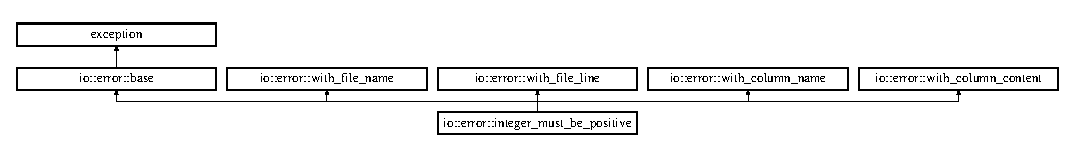
\includegraphics[height=1.577465cm]{structio_1_1error_1_1integer__must__be__positive}
\end{center}
\end{figure}
\subsection*{Public Member Functions}
\begin{DoxyCompactItemize}
\item 
\mbox{\Hypertarget{structio_1_1error_1_1integer__must__be__positive_af6daaa02512141958a3eafd0c07232ef}\label{structio_1_1error_1_1integer__must__be__positive_af6daaa02512141958a3eafd0c07232ef}} 
void {\bfseries format\+\_\+error\+\_\+message} () const
\end{DoxyCompactItemize}
\subsection*{Additional Inherited Members}


The documentation for this struct was generated from the following file\+:\begin{DoxyCompactItemize}
\item 
library/csv.\+h\end{DoxyCompactItemize}

\hypertarget{structio_1_1error_1_1integer__overflow}{}\section{io\+:\+:error\+:\+:integer\+\_\+overflow Struct Reference}
\label{structio_1_1error_1_1integer__overflow}\index{io\+::error\+::integer\+\_\+overflow@{io\+::error\+::integer\+\_\+overflow}}
Inheritance diagram for io\+:\+:error\+:\+:integer\+\_\+overflow\+:\begin{figure}[H]
\begin{center}
\leavevmode
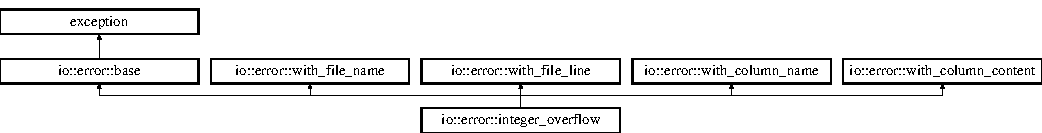
\includegraphics[height=1.787234cm]{structio_1_1error_1_1integer__overflow}
\end{center}
\end{figure}
\subsection*{Public Member Functions}
\begin{DoxyCompactItemize}
\item 
\mbox{\Hypertarget{structio_1_1error_1_1integer__overflow_a25825600c3c29210160ba201519e6312}\label{structio_1_1error_1_1integer__overflow_a25825600c3c29210160ba201519e6312}} 
void {\bfseries format\+\_\+error\+\_\+message} () const
\end{DoxyCompactItemize}
\subsection*{Additional Inherited Members}


The documentation for this struct was generated from the following file\+:\begin{DoxyCompactItemize}
\item 
library/csv.\+h\end{DoxyCompactItemize}

\hypertarget{structio_1_1error_1_1integer__underflow}{}\section{io\+:\+:error\+:\+:integer\+\_\+underflow Struct Reference}
\label{structio_1_1error_1_1integer__underflow}\index{io\+::error\+::integer\+\_\+underflow@{io\+::error\+::integer\+\_\+underflow}}
Inheritance diagram for io\+:\+:error\+:\+:integer\+\_\+underflow\+:\begin{figure}[H]
\begin{center}
\leavevmode
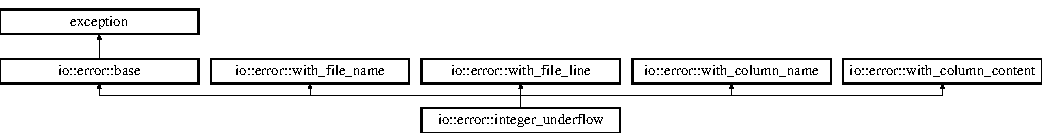
\includegraphics[height=1.787234cm]{structio_1_1error_1_1integer__underflow}
\end{center}
\end{figure}
\subsection*{Public Member Functions}
\begin{DoxyCompactItemize}
\item 
\mbox{\Hypertarget{structio_1_1error_1_1integer__underflow_a2ded9c7e982403877055514543207847}\label{structio_1_1error_1_1integer__underflow_a2ded9c7e982403877055514543207847}} 
void {\bfseries format\+\_\+error\+\_\+message} () const
\end{DoxyCompactItemize}
\subsection*{Additional Inherited Members}


The documentation for this struct was generated from the following file\+:\begin{DoxyCompactItemize}
\item 
library/csv.\+h\end{DoxyCompactItemize}

\hypertarget{structio_1_1error_1_1invalid__single__character}{}\section{io\+:\+:error\+:\+:invalid\+\_\+single\+\_\+character Struct Reference}
\label{structio_1_1error_1_1invalid__single__character}\index{io\+::error\+::invalid\+\_\+single\+\_\+character@{io\+::error\+::invalid\+\_\+single\+\_\+character}}
Inheritance diagram for io\+:\+:error\+:\+:invalid\+\_\+single\+\_\+character\+:\begin{figure}[H]
\begin{center}
\leavevmode
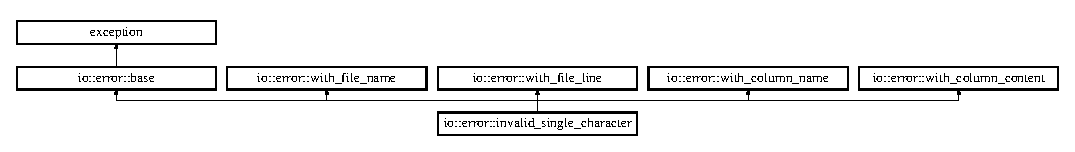
\includegraphics[height=1.600000cm]{structio_1_1error_1_1invalid__single__character}
\end{center}
\end{figure}
\subsection*{Public Member Functions}
\begin{DoxyCompactItemize}
\item 
\mbox{\Hypertarget{structio_1_1error_1_1invalid__single__character_a074ab35a8013ad15041a9bb9188e69bf}\label{structio_1_1error_1_1invalid__single__character_a074ab35a8013ad15041a9bb9188e69bf}} 
void {\bfseries format\+\_\+error\+\_\+message} () const
\end{DoxyCompactItemize}
\subsection*{Additional Inherited Members}


The documentation for this struct was generated from the following file\+:\begin{DoxyCompactItemize}
\item 
library/csv.\+h\end{DoxyCompactItemize}

\hypertarget{structio_1_1error_1_1line__length__limit__exceeded}{}\section{io\+:\+:error\+:\+:line\+\_\+length\+\_\+limit\+\_\+exceeded Struct Reference}
\label{structio_1_1error_1_1line__length__limit__exceeded}\index{io\+::error\+::line\+\_\+length\+\_\+limit\+\_\+exceeded@{io\+::error\+::line\+\_\+length\+\_\+limit\+\_\+exceeded}}
Inheritance diagram for io\+:\+:error\+:\+:line\+\_\+length\+\_\+limit\+\_\+exceeded\+:\begin{figure}[H]
\begin{center}
\leavevmode
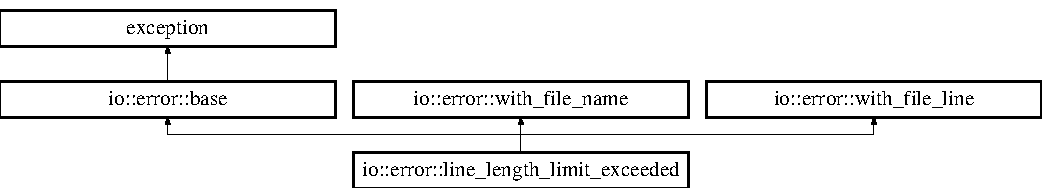
\includegraphics[height=2.522523cm]{structio_1_1error_1_1line__length__limit__exceeded}
\end{center}
\end{figure}
\subsection*{Public Member Functions}
\begin{DoxyCompactItemize}
\item 
\mbox{\Hypertarget{structio_1_1error_1_1line__length__limit__exceeded_ae6ef1cf3ed1d82804953ac120892b85e}\label{structio_1_1error_1_1line__length__limit__exceeded_ae6ef1cf3ed1d82804953ac120892b85e}} 
void {\bfseries format\+\_\+error\+\_\+message} () const
\end{DoxyCompactItemize}
\subsection*{Additional Inherited Members}


The documentation for this struct was generated from the following file\+:\begin{DoxyCompactItemize}
\item 
library/csv.\+h\end{DoxyCompactItemize}

\hypertarget{classio_1_1LineReader}{}\section{io\+:\+:Line\+Reader Class Reference}
\label{classio_1_1LineReader}\index{io\+::\+Line\+Reader@{io\+::\+Line\+Reader}}
\subsection*{Public Member Functions}
\begin{DoxyCompactItemize}
\item 
\mbox{\Hypertarget{classio_1_1LineReader_a84f2957de769bb701eaaddfd8bc004dd}\label{classio_1_1LineReader_a84f2957de769bb701eaaddfd8bc004dd}} 
{\bfseries Line\+Reader} (const \hyperlink{classio_1_1LineReader}{Line\+Reader} \&)=delete
\item 
\mbox{\Hypertarget{classio_1_1LineReader_a9ebd7beca16060ffc0ea8df3c0c6ff25}\label{classio_1_1LineReader_a9ebd7beca16060ffc0ea8df3c0c6ff25}} 
\hyperlink{classio_1_1LineReader}{Line\+Reader} \& {\bfseries operator=} (const \hyperlink{classio_1_1LineReader}{Line\+Reader} \&)=delete
\item 
\mbox{\Hypertarget{classio_1_1LineReader_a81a75d3f53725d35822f490007520e29}\label{classio_1_1LineReader_a81a75d3f53725d35822f490007520e29}} 
{\bfseries Line\+Reader} (const char $\ast$file\+\_\+name)
\item 
\mbox{\Hypertarget{classio_1_1LineReader_ab0eb26f44fa6b18f9c39dfb2561ac882}\label{classio_1_1LineReader_ab0eb26f44fa6b18f9c39dfb2561ac882}} 
{\bfseries Line\+Reader} (const std\+::string \&file\+\_\+name)
\item 
\mbox{\Hypertarget{classio_1_1LineReader_af4ebb130a7d6c78356573f6d0304266c}\label{classio_1_1LineReader_af4ebb130a7d6c78356573f6d0304266c}} 
{\bfseries Line\+Reader} (const char $\ast$file\+\_\+name, std\+::unique\+\_\+ptr$<$ \hyperlink{classio_1_1ByteSourceBase}{Byte\+Source\+Base} $>$byte\+\_\+source)
\item 
\mbox{\Hypertarget{classio_1_1LineReader_ab625b3a8001dca811b0e211c6cfc1b28}\label{classio_1_1LineReader_ab625b3a8001dca811b0e211c6cfc1b28}} 
{\bfseries Line\+Reader} (const std\+::string \&file\+\_\+name, std\+::unique\+\_\+ptr$<$ \hyperlink{classio_1_1ByteSourceBase}{Byte\+Source\+Base} $>$byte\+\_\+source)
\item 
\mbox{\Hypertarget{classio_1_1LineReader_ad5a65d6f23474884061a77ea858c042b}\label{classio_1_1LineReader_ad5a65d6f23474884061a77ea858c042b}} 
{\bfseries Line\+Reader} (const char $\ast$file\+\_\+name, const char $\ast$data\+\_\+begin, const char $\ast$data\+\_\+end)
\item 
\mbox{\Hypertarget{classio_1_1LineReader_a0a52d864b46442a253443cac1367366e}\label{classio_1_1LineReader_a0a52d864b46442a253443cac1367366e}} 
{\bfseries Line\+Reader} (const std\+::string \&file\+\_\+name, const char $\ast$data\+\_\+begin, const char $\ast$data\+\_\+end)
\item 
\mbox{\Hypertarget{classio_1_1LineReader_ad2a8943ba0848ae5052e2f5ad30c010e}\label{classio_1_1LineReader_ad2a8943ba0848ae5052e2f5ad30c010e}} 
{\bfseries Line\+Reader} (const char $\ast$file\+\_\+name, F\+I\+LE $\ast$file)
\item 
\mbox{\Hypertarget{classio_1_1LineReader_a93fa2e3ae98b0e7a7391714d6395c552}\label{classio_1_1LineReader_a93fa2e3ae98b0e7a7391714d6395c552}} 
{\bfseries Line\+Reader} (const std\+::string \&file\+\_\+name, F\+I\+LE $\ast$file)
\item 
\mbox{\Hypertarget{classio_1_1LineReader_a301c08eb9ca5d3fdccf4e9a8e5ac82f8}\label{classio_1_1LineReader_a301c08eb9ca5d3fdccf4e9a8e5ac82f8}} 
{\bfseries Line\+Reader} (const char $\ast$file\+\_\+name, std\+::istream \&in)
\item 
\mbox{\Hypertarget{classio_1_1LineReader_a3eacf4d1539a24122c6897fce4e72f06}\label{classio_1_1LineReader_a3eacf4d1539a24122c6897fce4e72f06}} 
{\bfseries Line\+Reader} (const std\+::string \&file\+\_\+name, std\+::istream \&in)
\item 
\mbox{\Hypertarget{classio_1_1LineReader_a1a0763d491dec16cebc33134e965dfee}\label{classio_1_1LineReader_a1a0763d491dec16cebc33134e965dfee}} 
void {\bfseries set\+\_\+file\+\_\+name} (const std\+::string \&file\+\_\+name)
\item 
\mbox{\Hypertarget{classio_1_1LineReader_a81c56ac68497da5ec874333ce063fd83}\label{classio_1_1LineReader_a81c56ac68497da5ec874333ce063fd83}} 
void {\bfseries set\+\_\+file\+\_\+name} (const char $\ast$file\+\_\+name)
\item 
\mbox{\Hypertarget{classio_1_1LineReader_ad5817da6af1ae77daddec7aeaeebf2f8}\label{classio_1_1LineReader_ad5817da6af1ae77daddec7aeaeebf2f8}} 
const char $\ast$ {\bfseries get\+\_\+truncated\+\_\+file\+\_\+name} () const
\item 
\mbox{\Hypertarget{classio_1_1LineReader_a581b55d4ced6adb964de50fa8ac6eb08}\label{classio_1_1LineReader_a581b55d4ced6adb964de50fa8ac6eb08}} 
void {\bfseries set\+\_\+file\+\_\+line} (unsigned file\+\_\+line)
\item 
\mbox{\Hypertarget{classio_1_1LineReader_a3f3459e22ed8e459238c290050b6722e}\label{classio_1_1LineReader_a3f3459e22ed8e459238c290050b6722e}} 
unsigned {\bfseries get\+\_\+file\+\_\+line} () const
\item 
\mbox{\Hypertarget{classio_1_1LineReader_a97f4e0129611d9da2b8c966ffe670be5}\label{classio_1_1LineReader_a97f4e0129611d9da2b8c966ffe670be5}} 
char $\ast$ {\bfseries next\+\_\+line} ()
\end{DoxyCompactItemize}
\subsection*{Private Member Functions}
\begin{DoxyCompactItemize}
\item 
\mbox{\Hypertarget{classio_1_1LineReader_a68ac92cedd46d25cbc4e205eb3a2833f}\label{classio_1_1LineReader_a68ac92cedd46d25cbc4e205eb3a2833f}} 
void {\bfseries init} (std\+::unique\+\_\+ptr$<$ \hyperlink{classio_1_1ByteSourceBase}{Byte\+Source\+Base} $>$byte\+\_\+source)
\end{DoxyCompactItemize}
\subsection*{Static Private Member Functions}
\begin{DoxyCompactItemize}
\item 
\mbox{\Hypertarget{classio_1_1LineReader_a036adce726096bca1db7ccceea938595}\label{classio_1_1LineReader_a036adce726096bca1db7ccceea938595}} 
static std\+::unique\+\_\+ptr$<$ \hyperlink{classio_1_1ByteSourceBase}{Byte\+Source\+Base} $>$ {\bfseries open\+\_\+file} (const char $\ast$file\+\_\+name)
\end{DoxyCompactItemize}
\subsection*{Private Attributes}
\begin{DoxyCompactItemize}
\item 
\mbox{\Hypertarget{classio_1_1LineReader_afd45c8f7175a4094a469f5764816d181}\label{classio_1_1LineReader_afd45c8f7175a4094a469f5764816d181}} 
std\+::unique\+\_\+ptr$<$ char\mbox{[}$\,$\mbox{]}$>$ {\bfseries buffer}
\item 
\mbox{\Hypertarget{classio_1_1LineReader_abfd04ef491b6515a26b1b17aab9430b0}\label{classio_1_1LineReader_abfd04ef491b6515a26b1b17aab9430b0}} 
\hyperlink{classio_1_1detail_1_1AsynchronousReader}{detail\+::\+Asynchronous\+Reader} {\bfseries reader}
\item 
\mbox{\Hypertarget{classio_1_1LineReader_a20676a014d14bfa566591d8cfeed0f29}\label{classio_1_1LineReader_a20676a014d14bfa566591d8cfeed0f29}} 
int {\bfseries data\+\_\+begin}
\item 
\mbox{\Hypertarget{classio_1_1LineReader_a16829b470aa908981d4799401d42a85b}\label{classio_1_1LineReader_a16829b470aa908981d4799401d42a85b}} 
int {\bfseries data\+\_\+end}
\item 
\mbox{\Hypertarget{classio_1_1LineReader_a8b853ac45c1eae0afc36d49630e949d8}\label{classio_1_1LineReader_a8b853ac45c1eae0afc36d49630e949d8}} 
char {\bfseries file\+\_\+name} \mbox{[}error\+::max\+\_\+file\+\_\+name\+\_\+length+1\mbox{]}
\item 
\mbox{\Hypertarget{classio_1_1LineReader_a5c29ad60208bca6475af54e54eff80b7}\label{classio_1_1LineReader_a5c29ad60208bca6475af54e54eff80b7}} 
unsigned {\bfseries file\+\_\+line}
\end{DoxyCompactItemize}
\subsection*{Static Private Attributes}
\begin{DoxyCompactItemize}
\item 
\mbox{\Hypertarget{classio_1_1LineReader_a04db9ad3b956347b48136dbe5751469d}\label{classio_1_1LineReader_a04db9ad3b956347b48136dbe5751469d}} 
static const int {\bfseries block\+\_\+len} = 1$<$$<$24
\end{DoxyCompactItemize}


The documentation for this class was generated from the following file\+:\begin{DoxyCompactItemize}
\item 
library/csv.\+h\end{DoxyCompactItemize}

\hypertarget{structio_1_1error_1_1missing__column__in__header}{}\section{io\+:\+:error\+:\+:missing\+\_\+column\+\_\+in\+\_\+header Struct Reference}
\label{structio_1_1error_1_1missing__column__in__header}\index{io\+::error\+::missing\+\_\+column\+\_\+in\+\_\+header@{io\+::error\+::missing\+\_\+column\+\_\+in\+\_\+header}}
Inheritance diagram for io\+:\+:error\+:\+:missing\+\_\+column\+\_\+in\+\_\+header\+:\begin{figure}[H]
\begin{center}
\leavevmode
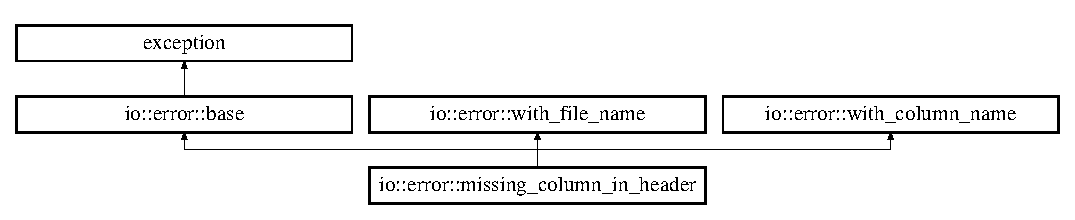
\includegraphics[height=2.511211cm]{structio_1_1error_1_1missing__column__in__header}
\end{center}
\end{figure}
\subsection*{Public Member Functions}
\begin{DoxyCompactItemize}
\item 
\mbox{\Hypertarget{structio_1_1error_1_1missing__column__in__header_a1a2bd4e01a389cb50c6bfae8443317fd}\label{structio_1_1error_1_1missing__column__in__header_a1a2bd4e01a389cb50c6bfae8443317fd}} 
void {\bfseries format\+\_\+error\+\_\+message} () const
\end{DoxyCompactItemize}
\subsection*{Additional Inherited Members}


The documentation for this struct was generated from the following file\+:\begin{DoxyCompactItemize}
\item 
library/csv.\+h\end{DoxyCompactItemize}

\hypertarget{structio_1_1no__comment}{}\section{io\+:\+:no\+\_\+comment Struct Reference}
\label{structio_1_1no__comment}\index{io\+::no\+\_\+comment@{io\+::no\+\_\+comment}}
\subsection*{Static Public Member Functions}
\begin{DoxyCompactItemize}
\item 
\mbox{\Hypertarget{structio_1_1no__comment_a52b252547482e28edd076ee2224bc8d8}\label{structio_1_1no__comment_a52b252547482e28edd076ee2224bc8d8}} 
static bool {\bfseries is\+\_\+comment} (const char $\ast$)
\end{DoxyCompactItemize}


The documentation for this struct was generated from the following file\+:\begin{DoxyCompactItemize}
\item 
library/csv.\+h\end{DoxyCompactItemize}

\hypertarget{structio_1_1error_1_1no__digit}{}\section{io\+:\+:error\+:\+:no\+\_\+digit Struct Reference}
\label{structio_1_1error_1_1no__digit}\index{io\+::error\+::no\+\_\+digit@{io\+::error\+::no\+\_\+digit}}
Inheritance diagram for io\+:\+:error\+:\+:no\+\_\+digit\+:\begin{figure}[H]
\begin{center}
\leavevmode
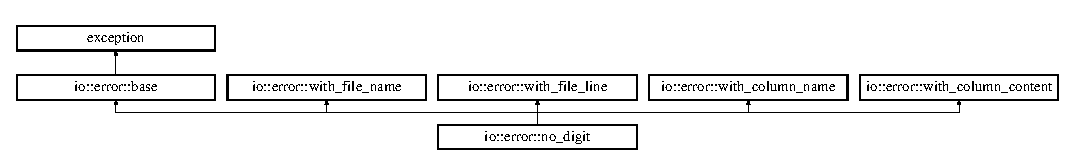
\includegraphics[height=1.787234cm]{structio_1_1error_1_1no__digit}
\end{center}
\end{figure}
\subsection*{Public Member Functions}
\begin{DoxyCompactItemize}
\item 
\mbox{\Hypertarget{structio_1_1error_1_1no__digit_a469275c63f67171903f9cdb2418da5b3}\label{structio_1_1error_1_1no__digit_a469275c63f67171903f9cdb2418da5b3}} 
void {\bfseries format\+\_\+error\+\_\+message} () const
\end{DoxyCompactItemize}
\subsection*{Additional Inherited Members}


The documentation for this struct was generated from the following file\+:\begin{DoxyCompactItemize}
\item 
library/csv.\+h\end{DoxyCompactItemize}

\hypertarget{structio_1_1no__quote__escape}{}\section{io\+:\+:no\+\_\+quote\+\_\+escape$<$ sep $>$ Struct Template Reference}
\label{structio_1_1no__quote__escape}\index{io\+::no\+\_\+quote\+\_\+escape$<$ sep $>$@{io\+::no\+\_\+quote\+\_\+escape$<$ sep $>$}}
\subsection*{Static Public Member Functions}
\begin{DoxyCompactItemize}
\item 
\mbox{\Hypertarget{structio_1_1no__quote__escape_add17b043bb89445079a0448026ce86d0}\label{structio_1_1no__quote__escape_add17b043bb89445079a0448026ce86d0}} 
static const char $\ast$ {\bfseries find\+\_\+next\+\_\+column\+\_\+end} (const char $\ast$col\+\_\+begin)
\item 
\mbox{\Hypertarget{structio_1_1no__quote__escape_af1c217f2c995d178a91c58235191b052}\label{structio_1_1no__quote__escape_af1c217f2c995d178a91c58235191b052}} 
static void {\bfseries unescape} (char $\ast$\&, char $\ast$\&)
\end{DoxyCompactItemize}


The documentation for this struct was generated from the following file\+:\begin{DoxyCompactItemize}
\item 
library/csv.\+h\end{DoxyCompactItemize}

\hypertarget{classio_1_1detail_1_1NonOwningIStreamByteSource}{}\section{io\+:\+:detail\+:\+:Non\+Owning\+I\+Stream\+Byte\+Source Class Reference}
\label{classio_1_1detail_1_1NonOwningIStreamByteSource}\index{io\+::detail\+::\+Non\+Owning\+I\+Stream\+Byte\+Source@{io\+::detail\+::\+Non\+Owning\+I\+Stream\+Byte\+Source}}
Inheritance diagram for io\+:\+:detail\+:\+:Non\+Owning\+I\+Stream\+Byte\+Source\+:\begin{figure}[H]
\begin{center}
\leavevmode
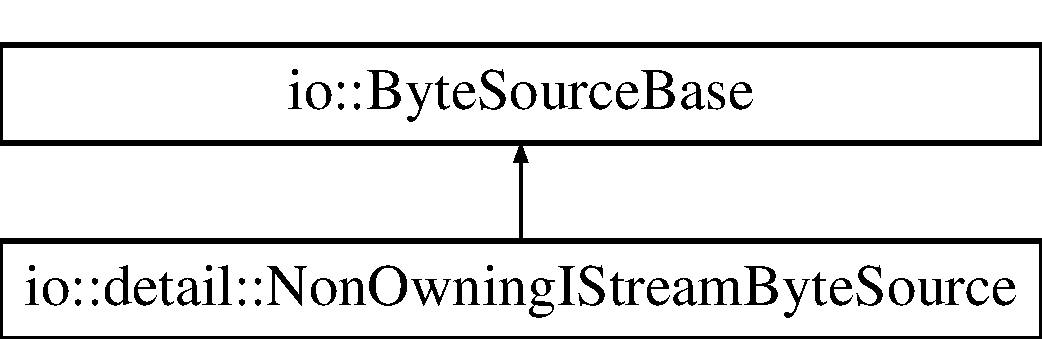
\includegraphics[height=2.000000cm]{classio_1_1detail_1_1NonOwningIStreamByteSource}
\end{center}
\end{figure}
\subsection*{Public Member Functions}
\begin{DoxyCompactItemize}
\item 
\mbox{\Hypertarget{classio_1_1detail_1_1NonOwningIStreamByteSource_aacb55ba2f52ba1c30810697d6aa92169}\label{classio_1_1detail_1_1NonOwningIStreamByteSource_aacb55ba2f52ba1c30810697d6aa92169}} 
{\bfseries Non\+Owning\+I\+Stream\+Byte\+Source} (std\+::istream \&in)
\item 
\mbox{\Hypertarget{classio_1_1detail_1_1NonOwningIStreamByteSource_ac7b1968c8314896d7ec0ebb97fdda30d}\label{classio_1_1detail_1_1NonOwningIStreamByteSource_ac7b1968c8314896d7ec0ebb97fdda30d}} 
int {\bfseries read} (char $\ast$buffer, int size)
\end{DoxyCompactItemize}
\subsection*{Private Attributes}
\begin{DoxyCompactItemize}
\item 
\mbox{\Hypertarget{classio_1_1detail_1_1NonOwningIStreamByteSource_a42ec07be9409b77a17bdf08cfa73739d}\label{classio_1_1detail_1_1NonOwningIStreamByteSource_a42ec07be9409b77a17bdf08cfa73739d}} 
std\+::istream \& {\bfseries in}
\end{DoxyCompactItemize}


The documentation for this class was generated from the following file\+:\begin{DoxyCompactItemize}
\item 
library/csv.\+h\end{DoxyCompactItemize}

\hypertarget{classio_1_1detail_1_1NonOwningStringByteSource}{}\section{io\+:\+:detail\+:\+:Non\+Owning\+String\+Byte\+Source Class Reference}
\label{classio_1_1detail_1_1NonOwningStringByteSource}\index{io\+::detail\+::\+Non\+Owning\+String\+Byte\+Source@{io\+::detail\+::\+Non\+Owning\+String\+Byte\+Source}}
Inheritance diagram for io\+:\+:detail\+:\+:Non\+Owning\+String\+Byte\+Source\+:\begin{figure}[H]
\begin{center}
\leavevmode
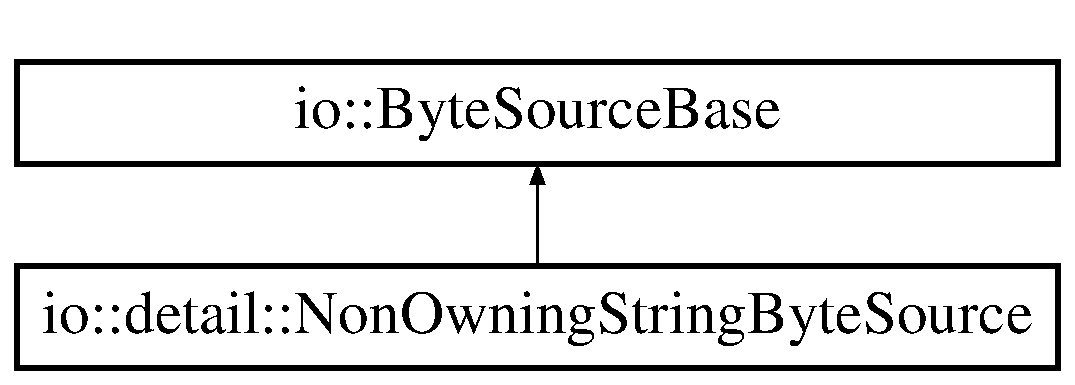
\includegraphics[height=2.000000cm]{classio_1_1detail_1_1NonOwningStringByteSource}
\end{center}
\end{figure}
\subsection*{Public Member Functions}
\begin{DoxyCompactItemize}
\item 
\mbox{\Hypertarget{classio_1_1detail_1_1NonOwningStringByteSource_a8fd604017b38e20f90386b6e10bd95a3}\label{classio_1_1detail_1_1NonOwningStringByteSource_a8fd604017b38e20f90386b6e10bd95a3}} 
{\bfseries Non\+Owning\+String\+Byte\+Source} (const char $\ast$str, long long size)
\item 
\mbox{\Hypertarget{classio_1_1detail_1_1NonOwningStringByteSource_aba194be7e3a141f40d683db483a620bb}\label{classio_1_1detail_1_1NonOwningStringByteSource_aba194be7e3a141f40d683db483a620bb}} 
int {\bfseries read} (char $\ast$buffer, int desired\+\_\+byte\+\_\+count)
\end{DoxyCompactItemize}
\subsection*{Private Attributes}
\begin{DoxyCompactItemize}
\item 
\mbox{\Hypertarget{classio_1_1detail_1_1NonOwningStringByteSource_ad130b4796eb5758c3e512d585af51bef}\label{classio_1_1detail_1_1NonOwningStringByteSource_ad130b4796eb5758c3e512d585af51bef}} 
const char $\ast$ {\bfseries str}
\item 
\mbox{\Hypertarget{classio_1_1detail_1_1NonOwningStringByteSource_aa2097ba0c3c49f0266ec1fbc8f322947}\label{classio_1_1detail_1_1NonOwningStringByteSource_aa2097ba0c3c49f0266ec1fbc8f322947}} 
long long {\bfseries remaining\+\_\+byte\+\_\+count}
\end{DoxyCompactItemize}


The documentation for this class was generated from the following file\+:\begin{DoxyCompactItemize}
\item 
library/csv.\+h\end{DoxyCompactItemize}

\hypertarget{classio_1_1detail_1_1OwningStdIOByteSourceBase}{}\section{io\+:\+:detail\+:\+:Owning\+Std\+I\+O\+Byte\+Source\+Base Class Reference}
\label{classio_1_1detail_1_1OwningStdIOByteSourceBase}\index{io\+::detail\+::\+Owning\+Std\+I\+O\+Byte\+Source\+Base@{io\+::detail\+::\+Owning\+Std\+I\+O\+Byte\+Source\+Base}}
Inheritance diagram for io\+:\+:detail\+:\+:Owning\+Std\+I\+O\+Byte\+Source\+Base\+:\begin{figure}[H]
\begin{center}
\leavevmode
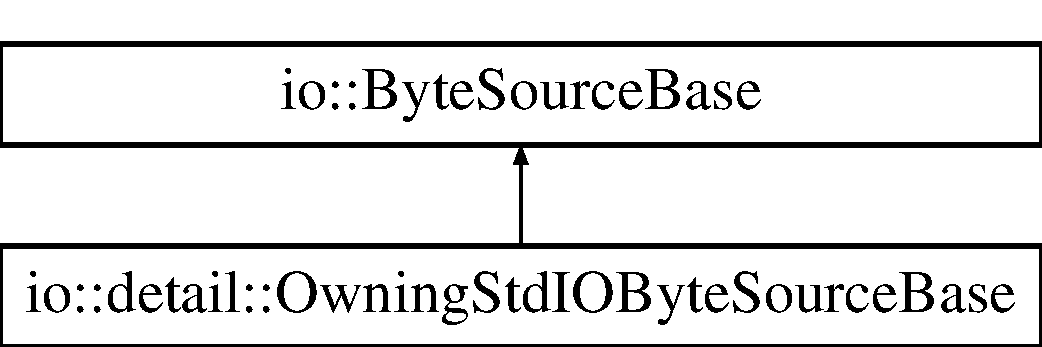
\includegraphics[height=2.000000cm]{classio_1_1detail_1_1OwningStdIOByteSourceBase}
\end{center}
\end{figure}
\subsection*{Public Member Functions}
\begin{DoxyCompactItemize}
\item 
\mbox{\Hypertarget{classio_1_1detail_1_1OwningStdIOByteSourceBase_a259f77d1a3c57720b54b88d9f8a3c018}\label{classio_1_1detail_1_1OwningStdIOByteSourceBase_a259f77d1a3c57720b54b88d9f8a3c018}} 
{\bfseries Owning\+Std\+I\+O\+Byte\+Source\+Base} (F\+I\+LE $\ast$file)
\item 
\mbox{\Hypertarget{classio_1_1detail_1_1OwningStdIOByteSourceBase_a9269e7bfd07ebf2fa3518912fe7bebd0}\label{classio_1_1detail_1_1OwningStdIOByteSourceBase_a9269e7bfd07ebf2fa3518912fe7bebd0}} 
int {\bfseries read} (char $\ast$buffer, int size)
\end{DoxyCompactItemize}
\subsection*{Private Attributes}
\begin{DoxyCompactItemize}
\item 
\mbox{\Hypertarget{classio_1_1detail_1_1OwningStdIOByteSourceBase_a00f62c8522d0fe9edadf3d094e94ae26}\label{classio_1_1detail_1_1OwningStdIOByteSourceBase_a00f62c8522d0fe9edadf3d094e94ae26}} 
F\+I\+LE $\ast$ {\bfseries file}
\end{DoxyCompactItemize}


The documentation for this class was generated from the following file\+:\begin{DoxyCompactItemize}
\item 
library/csv.\+h\end{DoxyCompactItemize}

\hypertarget{structio_1_1set__to__max__on__overflow}{}\section{io\+:\+:set\+\_\+to\+\_\+max\+\_\+on\+\_\+overflow Struct Reference}
\label{structio_1_1set__to__max__on__overflow}\index{io\+::set\+\_\+to\+\_\+max\+\_\+on\+\_\+overflow@{io\+::set\+\_\+to\+\_\+max\+\_\+on\+\_\+overflow}}
\subsection*{Static Public Member Functions}
\begin{DoxyCompactItemize}
\item 
\mbox{\Hypertarget{structio_1_1set__to__max__on__overflow_a770dee97a1ee55131163e6be8d4c0d9d}\label{structio_1_1set__to__max__on__overflow_a770dee97a1ee55131163e6be8d4c0d9d}} 
{\footnotesize template$<$class T $>$ }\\static void {\bfseries on\+\_\+overflow} (T \&x)
\item 
\mbox{\Hypertarget{structio_1_1set__to__max__on__overflow_a812d316e2b23247df19ca83bfda90a59}\label{structio_1_1set__to__max__on__overflow_a812d316e2b23247df19ca83bfda90a59}} 
{\footnotesize template$<$class T $>$ }\\static void {\bfseries on\+\_\+underflow} (T \&x)
\end{DoxyCompactItemize}


The documentation for this struct was generated from the following file\+:\begin{DoxyCompactItemize}
\item 
library/csv.\+h\end{DoxyCompactItemize}

\hypertarget{structio_1_1single__and__empty__line__comment}{}\section{io\+:\+:single\+\_\+and\+\_\+empty\+\_\+line\+\_\+comment$<$ comment\+\_\+start\+\_\+char\+\_\+list $>$ Struct Template Reference}
\label{structio_1_1single__and__empty__line__comment}\index{io\+::single\+\_\+and\+\_\+empty\+\_\+line\+\_\+comment$<$ comment\+\_\+start\+\_\+char\+\_\+list $>$@{io\+::single\+\_\+and\+\_\+empty\+\_\+line\+\_\+comment$<$ comment\+\_\+start\+\_\+char\+\_\+list $>$}}
\subsection*{Static Public Member Functions}
\begin{DoxyCompactItemize}
\item 
\mbox{\Hypertarget{structio_1_1single__and__empty__line__comment_a93a1556dfe4d7e6e3a674d576c4b30f4}\label{structio_1_1single__and__empty__line__comment_a93a1556dfe4d7e6e3a674d576c4b30f4}} 
static bool {\bfseries is\+\_\+comment} (const char $\ast$line)
\end{DoxyCompactItemize}


The documentation for this struct was generated from the following file\+:\begin{DoxyCompactItemize}
\item 
library/csv.\+h\end{DoxyCompactItemize}

\hypertarget{structio_1_1single__line__comment}{}\section{io\+:\+:single\+\_\+line\+\_\+comment$<$ comment\+\_\+start\+\_\+char\+\_\+list $>$ Struct Template Reference}
\label{structio_1_1single__line__comment}\index{io\+::single\+\_\+line\+\_\+comment$<$ comment\+\_\+start\+\_\+char\+\_\+list $>$@{io\+::single\+\_\+line\+\_\+comment$<$ comment\+\_\+start\+\_\+char\+\_\+list $>$}}
\subsection*{Static Public Member Functions}
\begin{DoxyCompactItemize}
\item 
\mbox{\Hypertarget{structio_1_1single__line__comment_ac4b029bb0efd251505f8e610cc308a92}\label{structio_1_1single__line__comment_ac4b029bb0efd251505f8e610cc308a92}} 
static bool {\bfseries is\+\_\+comment} (const char $\ast$line)
\end{DoxyCompactItemize}
\subsection*{Static Private Member Functions}
\begin{DoxyCompactItemize}
\item 
\mbox{\Hypertarget{structio_1_1single__line__comment_a961a1b5c85dd2ec717ff483cb2206ade}\label{structio_1_1single__line__comment_a961a1b5c85dd2ec717ff483cb2206ade}} 
static constexpr bool {\bfseries is\+\_\+comment\+\_\+start\+\_\+char} (char)
\item 
\mbox{\Hypertarget{structio_1_1single__line__comment_a9533453f729d2216f52af087e4411548}\label{structio_1_1single__line__comment_a9533453f729d2216f52af087e4411548}} 
{\footnotesize template$<$class ... Other\+Comment\+Start\+Chars$>$ }\\static constexpr bool {\bfseries is\+\_\+comment\+\_\+start\+\_\+char} (char c, char comment\+\_\+start\+\_\+char, Other\+Comment\+Start\+Chars...\+other\+\_\+comment\+\_\+start\+\_\+chars)
\end{DoxyCompactItemize}


The documentation for this struct was generated from the following file\+:\begin{DoxyCompactItemize}
\item 
library/csv.\+h\end{DoxyCompactItemize}

\hypertarget{classio_1_1detail_1_1SynchronousReader}{}\section{io\+:\+:detail\+:\+:Synchronous\+Reader Class Reference}
\label{classio_1_1detail_1_1SynchronousReader}\index{io\+::detail\+::\+Synchronous\+Reader@{io\+::detail\+::\+Synchronous\+Reader}}
\subsection*{Public Member Functions}
\begin{DoxyCompactItemize}
\item 
\mbox{\Hypertarget{classio_1_1detail_1_1SynchronousReader_a4dc78563ff667b92ad3096a94e834eb5}\label{classio_1_1detail_1_1SynchronousReader_a4dc78563ff667b92ad3096a94e834eb5}} 
void {\bfseries init} (std\+::unique\+\_\+ptr$<$ \hyperlink{classio_1_1ByteSourceBase}{Byte\+Source\+Base} $>$arg\+\_\+byte\+\_\+source)
\item 
\mbox{\Hypertarget{classio_1_1detail_1_1SynchronousReader_a9d6b2c888cc7020df1bb81c8bb5c58bc}\label{classio_1_1detail_1_1SynchronousReader_a9d6b2c888cc7020df1bb81c8bb5c58bc}} 
bool {\bfseries is\+\_\+valid} () const
\item 
\mbox{\Hypertarget{classio_1_1detail_1_1SynchronousReader_a6cad1371b97e14f660914898b16433c4}\label{classio_1_1detail_1_1SynchronousReader_a6cad1371b97e14f660914898b16433c4}} 
void {\bfseries start\+\_\+read} (char $\ast$arg\+\_\+buffer, int arg\+\_\+desired\+\_\+byte\+\_\+count)
\item 
\mbox{\Hypertarget{classio_1_1detail_1_1SynchronousReader_a519a0cb25c641d2e51b6542749c44606}\label{classio_1_1detail_1_1SynchronousReader_a519a0cb25c641d2e51b6542749c44606}} 
int {\bfseries finish\+\_\+read} ()
\end{DoxyCompactItemize}
\subsection*{Private Attributes}
\begin{DoxyCompactItemize}
\item 
\mbox{\Hypertarget{classio_1_1detail_1_1SynchronousReader_aa4ab4d5029b7d438051b4c800292059d}\label{classio_1_1detail_1_1SynchronousReader_aa4ab4d5029b7d438051b4c800292059d}} 
std\+::unique\+\_\+ptr$<$ \hyperlink{classio_1_1ByteSourceBase}{Byte\+Source\+Base} $>$ {\bfseries byte\+\_\+source}
\item 
\mbox{\Hypertarget{classio_1_1detail_1_1SynchronousReader_aa57e237e05bd90abdd9e896647da3fc7}\label{classio_1_1detail_1_1SynchronousReader_aa57e237e05bd90abdd9e896647da3fc7}} 
char $\ast$ {\bfseries buffer}
\item 
\mbox{\Hypertarget{classio_1_1detail_1_1SynchronousReader_ac85e7a1b24cd383fb9fbfafe648f9ad6}\label{classio_1_1detail_1_1SynchronousReader_ac85e7a1b24cd383fb9fbfafe648f9ad6}} 
int {\bfseries desired\+\_\+byte\+\_\+count}
\end{DoxyCompactItemize}


The documentation for this class was generated from the following file\+:\begin{DoxyCompactItemize}
\item 
library/csv.\+h\end{DoxyCompactItemize}

\hypertarget{structio_1_1throw__on__overflow}{}\section{io\+:\+:throw\+\_\+on\+\_\+overflow Struct Reference}
\label{structio_1_1throw__on__overflow}\index{io\+::throw\+\_\+on\+\_\+overflow@{io\+::throw\+\_\+on\+\_\+overflow}}
\subsection*{Static Public Member Functions}
\begin{DoxyCompactItemize}
\item 
\mbox{\Hypertarget{structio_1_1throw__on__overflow_a0a59c1dc2ead1a9275c62885ec7545d2}\label{structio_1_1throw__on__overflow_a0a59c1dc2ead1a9275c62885ec7545d2}} 
{\footnotesize template$<$class T $>$ }\\static void {\bfseries on\+\_\+overflow} (T \&)
\item 
\mbox{\Hypertarget{structio_1_1throw__on__overflow_a2ae91b1ae3d655c16f7e6a7e9a1abd92}\label{structio_1_1throw__on__overflow_a2ae91b1ae3d655c16f7e6a7e9a1abd92}} 
{\footnotesize template$<$class T $>$ }\\static void {\bfseries on\+\_\+underflow} (T \&)
\end{DoxyCompactItemize}


The documentation for this struct was generated from the following file\+:\begin{DoxyCompactItemize}
\item 
library/csv.\+h\end{DoxyCompactItemize}

\hypertarget{structio_1_1error_1_1too__few__columns}{}\section{io\+:\+:error\+:\+:too\+\_\+few\+\_\+columns Struct Reference}
\label{structio_1_1error_1_1too__few__columns}\index{io\+::error\+::too\+\_\+few\+\_\+columns@{io\+::error\+::too\+\_\+few\+\_\+columns}}
Inheritance diagram for io\+:\+:error\+:\+:too\+\_\+few\+\_\+columns\+:\begin{figure}[H]
\begin{center}
\leavevmode
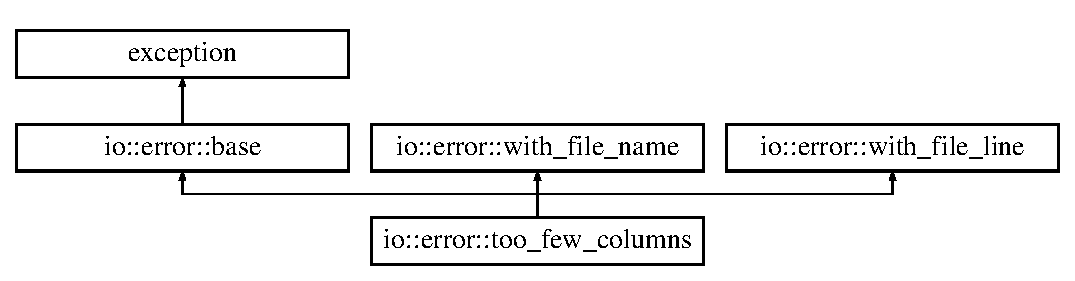
\includegraphics[height=3.000000cm]{structio_1_1error_1_1too__few__columns}
\end{center}
\end{figure}
\subsection*{Public Member Functions}
\begin{DoxyCompactItemize}
\item 
\mbox{\Hypertarget{structio_1_1error_1_1too__few__columns_a58d6d1fada127120facbcc00851ab455}\label{structio_1_1error_1_1too__few__columns_a58d6d1fada127120facbcc00851ab455}} 
void {\bfseries format\+\_\+error\+\_\+message} () const
\end{DoxyCompactItemize}
\subsection*{Additional Inherited Members}


The documentation for this struct was generated from the following file\+:\begin{DoxyCompactItemize}
\item 
library/csv.\+h\end{DoxyCompactItemize}

\hypertarget{structio_1_1error_1_1too__many__columns}{}\section{io\+:\+:error\+:\+:too\+\_\+many\+\_\+columns Struct Reference}
\label{structio_1_1error_1_1too__many__columns}\index{io\+::error\+::too\+\_\+many\+\_\+columns@{io\+::error\+::too\+\_\+many\+\_\+columns}}
Inheritance diagram for io\+:\+:error\+:\+:too\+\_\+many\+\_\+columns\+:\begin{figure}[H]
\begin{center}
\leavevmode
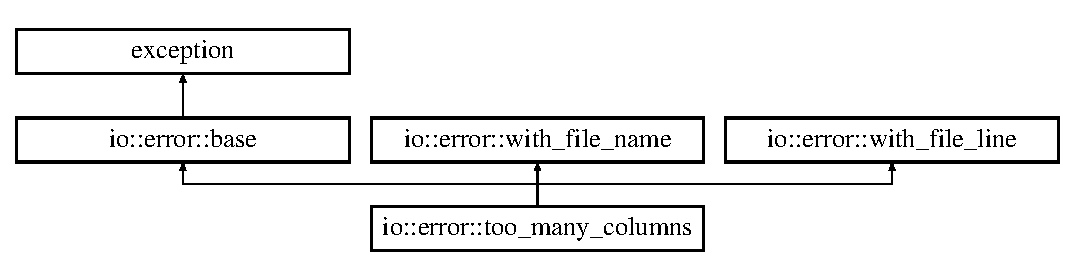
\includegraphics[height=3.000000cm]{structio_1_1error_1_1too__many__columns}
\end{center}
\end{figure}
\subsection*{Public Member Functions}
\begin{DoxyCompactItemize}
\item 
\mbox{\Hypertarget{structio_1_1error_1_1too__many__columns_a2072af07b0408387579becc076a9809e}\label{structio_1_1error_1_1too__many__columns_a2072af07b0408387579becc076a9809e}} 
void {\bfseries format\+\_\+error\+\_\+message} () const
\end{DoxyCompactItemize}
\subsection*{Additional Inherited Members}


The documentation for this struct was generated from the following file\+:\begin{DoxyCompactItemize}
\item 
library/csv.\+h\end{DoxyCompactItemize}

\hypertarget{structio_1_1trim__chars}{}\section{io\+:\+:trim\+\_\+chars$<$ trim\+\_\+char\+\_\+list $>$ Struct Template Reference}
\label{structio_1_1trim__chars}\index{io\+::trim\+\_\+chars$<$ trim\+\_\+char\+\_\+list $>$@{io\+::trim\+\_\+chars$<$ trim\+\_\+char\+\_\+list $>$}}
\subsection*{Static Public Member Functions}
\begin{DoxyCompactItemize}
\item 
\mbox{\Hypertarget{structio_1_1trim__chars_a4cffc5e839ab4024ca8c8330e26e338c}\label{structio_1_1trim__chars_a4cffc5e839ab4024ca8c8330e26e338c}} 
static void {\bfseries trim} (char $\ast$\&str\+\_\+begin, char $\ast$\&str\+\_\+end)
\end{DoxyCompactItemize}
\subsection*{Static Private Member Functions}
\begin{DoxyCompactItemize}
\item 
\mbox{\Hypertarget{structio_1_1trim__chars_a8868df0aa3887f5968cab2fac9c746fb}\label{structio_1_1trim__chars_a8868df0aa3887f5968cab2fac9c746fb}} 
static constexpr bool {\bfseries is\+\_\+trim\+\_\+char} (char)
\item 
\mbox{\Hypertarget{structio_1_1trim__chars_a4c365acae57f96990d08e9b4c6a89e48}\label{structio_1_1trim__chars_a4c365acae57f96990d08e9b4c6a89e48}} 
{\footnotesize template$<$class ... Other\+Trim\+Chars$>$ }\\static constexpr bool {\bfseries is\+\_\+trim\+\_\+char} (char c, char trim\+\_\+char, Other\+Trim\+Chars...\+other\+\_\+trim\+\_\+chars)
\end{DoxyCompactItemize}


The documentation for this struct was generated from the following file\+:\begin{DoxyCompactItemize}
\item 
library/csv.\+h\end{DoxyCompactItemize}

\hypertarget{structio_1_1error_1_1with__column__content}{}\section{io\+:\+:error\+:\+:with\+\_\+column\+\_\+content Struct Reference}
\label{structio_1_1error_1_1with__column__content}\index{io\+::error\+::with\+\_\+column\+\_\+content@{io\+::error\+::with\+\_\+column\+\_\+content}}
Inheritance diagram for io\+:\+:error\+:\+:with\+\_\+column\+\_\+content\+:\begin{figure}[H]
\begin{center}
\leavevmode
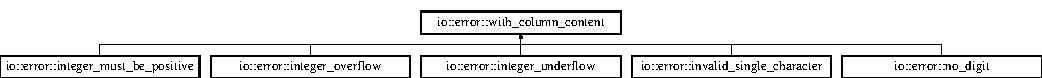
\includegraphics[height=1.051643cm]{structio_1_1error_1_1with__column__content}
\end{center}
\end{figure}
\subsection*{Public Member Functions}
\begin{DoxyCompactItemize}
\item 
\mbox{\Hypertarget{structio_1_1error_1_1with__column__content_ae7375310dc02425cb3cc4115b3ac8d6a}\label{structio_1_1error_1_1with__column__content_ae7375310dc02425cb3cc4115b3ac8d6a}} 
void {\bfseries set\+\_\+column\+\_\+content} (const char $\ast$column\+\_\+content)
\end{DoxyCompactItemize}
\subsection*{Public Attributes}
\begin{DoxyCompactItemize}
\item 
\mbox{\Hypertarget{structio_1_1error_1_1with__column__content_a8587779769fbfb40155abb362137a523}\label{structio_1_1error_1_1with__column__content_a8587779769fbfb40155abb362137a523}} 
char {\bfseries column\+\_\+content} \mbox{[}max\+\_\+column\+\_\+content\+\_\+length+1\mbox{]}
\end{DoxyCompactItemize}


The documentation for this struct was generated from the following file\+:\begin{DoxyCompactItemize}
\item 
library/csv.\+h\end{DoxyCompactItemize}

\hypertarget{structio_1_1error_1_1with__column__name}{}\section{io\+:\+:error\+:\+:with\+\_\+column\+\_\+name Struct Reference}
\label{structio_1_1error_1_1with__column__name}\index{io\+::error\+::with\+\_\+column\+\_\+name@{io\+::error\+::with\+\_\+column\+\_\+name}}
Inheritance diagram for io\+:\+:error\+:\+:with\+\_\+column\+\_\+name\+:\begin{figure}[H]
\begin{center}
\leavevmode
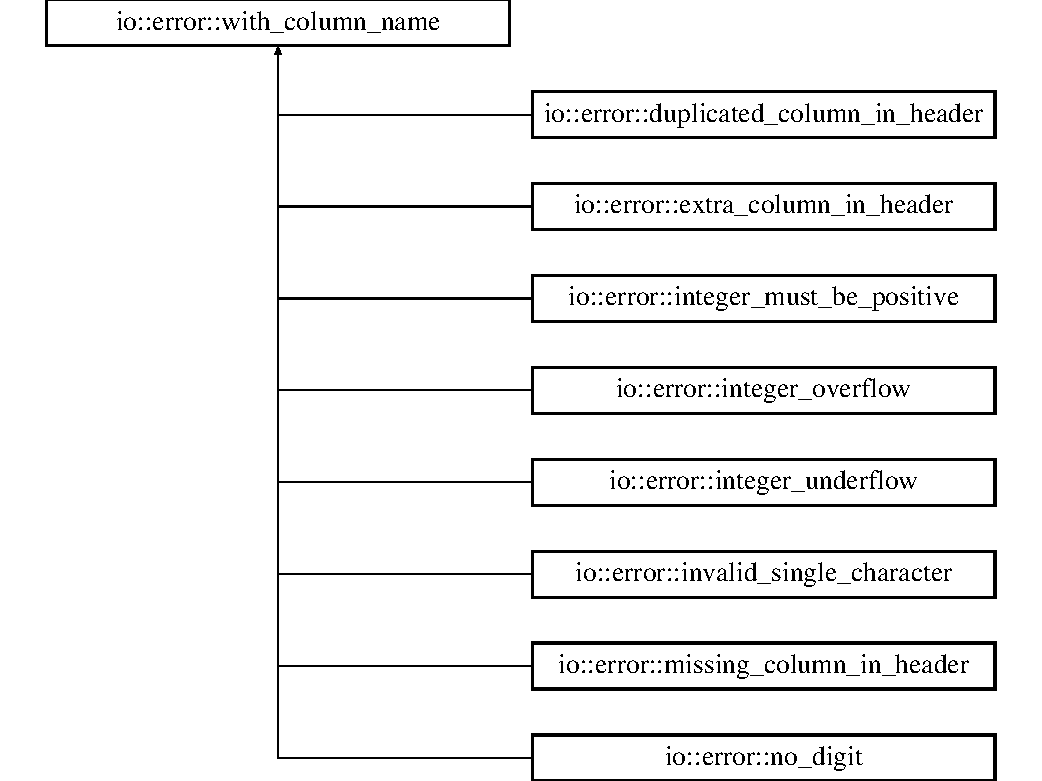
\includegraphics[height=9.000000cm]{structio_1_1error_1_1with__column__name}
\end{center}
\end{figure}
\subsection*{Public Member Functions}
\begin{DoxyCompactItemize}
\item 
\mbox{\Hypertarget{structio_1_1error_1_1with__column__name_a2a8144d3591a4bb618368ca7261befef}\label{structio_1_1error_1_1with__column__name_a2a8144d3591a4bb618368ca7261befef}} 
void {\bfseries set\+\_\+column\+\_\+name} (const char $\ast$column\+\_\+name)
\end{DoxyCompactItemize}
\subsection*{Public Attributes}
\begin{DoxyCompactItemize}
\item 
\mbox{\Hypertarget{structio_1_1error_1_1with__column__name_af40ba00f1f035d363b099baf1f724323}\label{structio_1_1error_1_1with__column__name_af40ba00f1f035d363b099baf1f724323}} 
char {\bfseries column\+\_\+name} \mbox{[}max\+\_\+column\+\_\+name\+\_\+length+1\mbox{]}
\end{DoxyCompactItemize}


The documentation for this struct was generated from the following file\+:\begin{DoxyCompactItemize}
\item 
library/csv.\+h\end{DoxyCompactItemize}

\hypertarget{structio_1_1error_1_1with__errno}{}\section{io\+:\+:error\+:\+:with\+\_\+errno Struct Reference}
\label{structio_1_1error_1_1with__errno}\index{io\+::error\+::with\+\_\+errno@{io\+::error\+::with\+\_\+errno}}
Inheritance diagram for io\+:\+:error\+:\+:with\+\_\+errno\+:\begin{figure}[H]
\begin{center}
\leavevmode
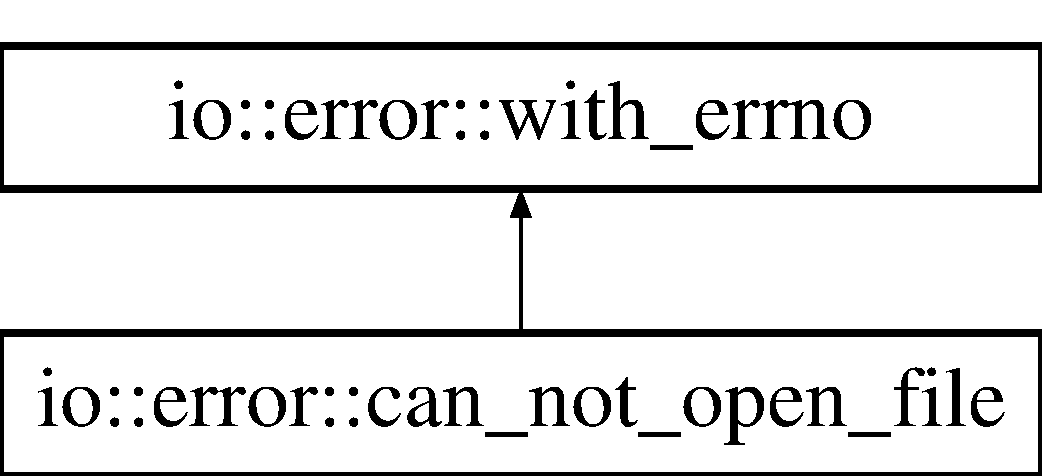
\includegraphics[height=2.000000cm]{structio_1_1error_1_1with__errno}
\end{center}
\end{figure}
\subsection*{Public Member Functions}
\begin{DoxyCompactItemize}
\item 
\mbox{\Hypertarget{structio_1_1error_1_1with__errno_a572cfa4b4a96792cd1d17dc9ad2eb5a9}\label{structio_1_1error_1_1with__errno_a572cfa4b4a96792cd1d17dc9ad2eb5a9}} 
void {\bfseries set\+\_\+errno} (int errno\+\_\+value)
\end{DoxyCompactItemize}
\subsection*{Public Attributes}
\begin{DoxyCompactItemize}
\item 
\mbox{\Hypertarget{structio_1_1error_1_1with__errno_a99dcacba02cb53351fe64d7e064406be}\label{structio_1_1error_1_1with__errno_a99dcacba02cb53351fe64d7e064406be}} 
int {\bfseries errno\+\_\+value}
\end{DoxyCompactItemize}


The documentation for this struct was generated from the following file\+:\begin{DoxyCompactItemize}
\item 
library/csv.\+h\end{DoxyCompactItemize}

\hypertarget{structio_1_1error_1_1with__file__line}{}\section{io\+:\+:error\+:\+:with\+\_\+file\+\_\+line Struct Reference}
\label{structio_1_1error_1_1with__file__line}\index{io\+::error\+::with\+\_\+file\+\_\+line@{io\+::error\+::with\+\_\+file\+\_\+line}}
Inheritance diagram for io\+:\+:error\+:\+:with\+\_\+file\+\_\+line\+:\begin{figure}[H]
\begin{center}
\leavevmode
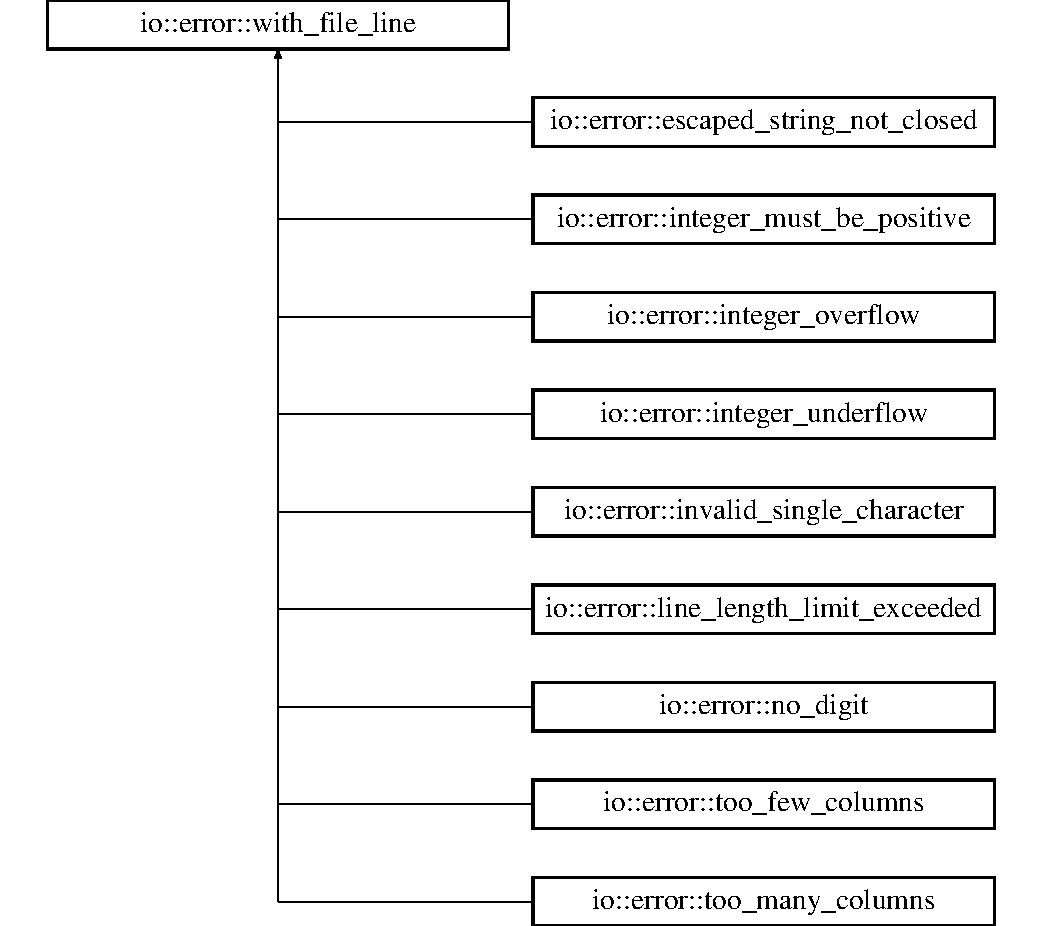
\includegraphics[height=10.000000cm]{structio_1_1error_1_1with__file__line}
\end{center}
\end{figure}
\subsection*{Public Member Functions}
\begin{DoxyCompactItemize}
\item 
\mbox{\Hypertarget{structio_1_1error_1_1with__file__line_aa92778a81778abc676ec6ee9952bba8c}\label{structio_1_1error_1_1with__file__line_aa92778a81778abc676ec6ee9952bba8c}} 
void {\bfseries set\+\_\+file\+\_\+line} (int file\+\_\+line)
\end{DoxyCompactItemize}
\subsection*{Public Attributes}
\begin{DoxyCompactItemize}
\item 
\mbox{\Hypertarget{structio_1_1error_1_1with__file__line_a391298c37172bcdb83aeb3daf65d5a0e}\label{structio_1_1error_1_1with__file__line_a391298c37172bcdb83aeb3daf65d5a0e}} 
int {\bfseries file\+\_\+line}
\end{DoxyCompactItemize}


The documentation for this struct was generated from the following file\+:\begin{DoxyCompactItemize}
\item 
library/csv.\+h\end{DoxyCompactItemize}

\hypertarget{structio_1_1error_1_1with__file__name}{}\section{io\+:\+:error\+:\+:with\+\_\+file\+\_\+name Struct Reference}
\label{structio_1_1error_1_1with__file__name}\index{io\+::error\+::with\+\_\+file\+\_\+name@{io\+::error\+::with\+\_\+file\+\_\+name}}
Inheritance diagram for io\+:\+:error\+:\+:with\+\_\+file\+\_\+name\+:\begin{figure}[H]
\begin{center}
\leavevmode
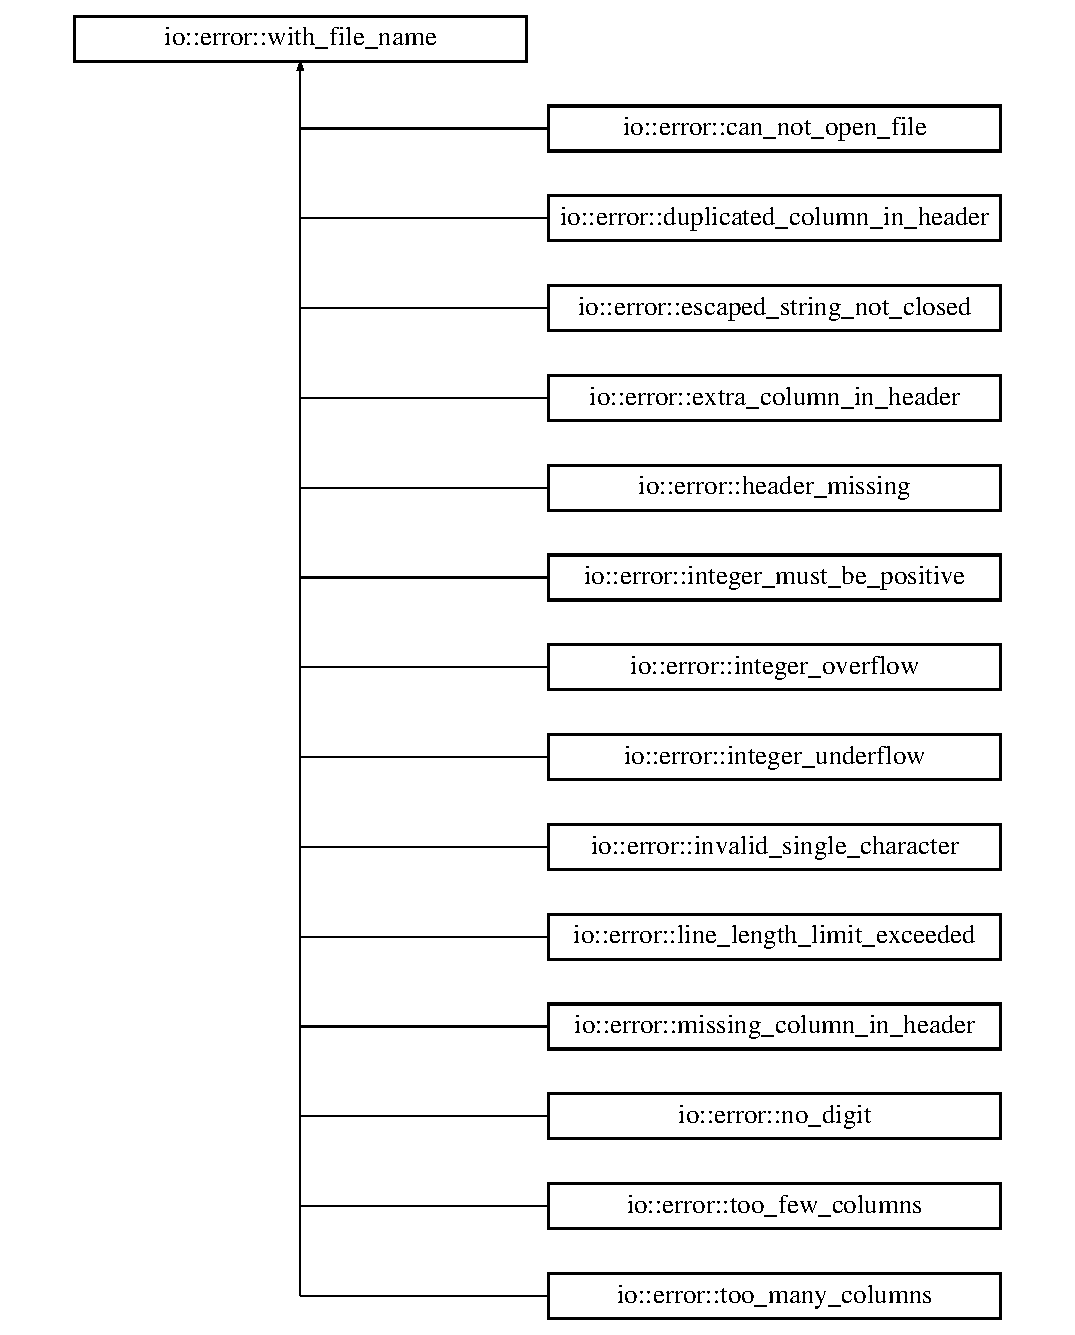
\includegraphics[height=12.000000cm]{structio_1_1error_1_1with__file__name}
\end{center}
\end{figure}
\subsection*{Public Member Functions}
\begin{DoxyCompactItemize}
\item 
\mbox{\Hypertarget{structio_1_1error_1_1with__file__name_ae765de62778c989d4658b4efe2995390}\label{structio_1_1error_1_1with__file__name_ae765de62778c989d4658b4efe2995390}} 
void {\bfseries set\+\_\+file\+\_\+name} (const char $\ast$file\+\_\+name)
\end{DoxyCompactItemize}
\subsection*{Public Attributes}
\begin{DoxyCompactItemize}
\item 
\mbox{\Hypertarget{structio_1_1error_1_1with__file__name_ac957d5590a8b95517b74eb5bf373a424}\label{structio_1_1error_1_1with__file__name_ac957d5590a8b95517b74eb5bf373a424}} 
char {\bfseries file\+\_\+name} \mbox{[}max\+\_\+file\+\_\+name\+\_\+length+1\mbox{]}
\end{DoxyCompactItemize}


The documentation for this struct was generated from the following file\+:\begin{DoxyCompactItemize}
\item 
library/csv.\+h\end{DoxyCompactItemize}

%--- End generated contents ---

% Index
\backmatter
\newpage
\phantomsection
\clearemptydoublepage
\addcontentsline{toc}{chapter}{Index}
\printindex

\end{document}
